\documentclass[conference]{IEEEtran}
\IEEEoverridecommandlockouts
% The preceding line is only needed to identify funding in the first footnote.
\usepackage{cite}
\usepackage{amsmath,amssymb,amsfonts}
\usepackage{algorithmic}
\usepackage{graphicx}
\usepackage{textcomp}
\usepackage{xcolor}
\usepackage[T1]{fontenc}
\def\BibTeX{{\rm B\kern-.05em{\sc i\kern-.025em b}\kern-.08em
    T\kern-.1667em\lower.7ex\hbox{E}\kern-.125emX}}
\begin{document}
\emergencystretch=3em

\title{Low-Resource ASR for Kalenjin: Two-Stage Fine-Tuning of Wav2Vec2-XLS-R with KenLM Integration

}

\author{
\IEEEauthorblockN{1\textsuperscript{st} Kevin Omondi Obote}
\IEEEauthorblockA{\textit{Strathmore Institute of} \\
\textit{Mathematical Sciences} \\
\textit{Strathmore University}\\
Nairobi, Kenya \\
kevin.obote@strathmore.edu}
\and
\IEEEauthorblockN{2\textsuperscript{nd} Annah Mumbua Muli}
\IEEEauthorblockA{\textit{Dept.\ of Languages} \\
\textit{and Linguistics} \\
\textit{Machakos University}\\
Machakos, Kenya \\
muliannah3@gmail.com}
\and
\IEEEauthorblockN{3\textsuperscript{rd} Vivian Nyamari Moraa}
\IEEEauthorblockA{\textit{Strathmore Institute of} \\
\textit{Mathematical Sciences} \\
\textit{Strathmore University}\\
Nairobi, Kenya \\
vnyamari@strathmore.edu}
\and
\IEEEauthorblockN{4\textsuperscript{th} Joyce Muthoni Njiiri}
\IEEEauthorblockA{\textit{Dept.\ of Languages} \\
\textit{and Linguistics} \\
\textit{Machakos University}\\
Machakos, Kenya \\
joycenjiiri@mksu.ac.ke}
}

\maketitle

\begin{abstract}
Automatic Speech Recognition (ASR) for under-resourced African languages remains a critical barrier to digital inclusion. This paper presents a comprehensive ASR framework for Kalenjin, a tonal, agglutinative Southern Nilotic language spoken by approximately 5--6 million people in Kenya's Rift Valley. We fine-tune Wav2Vec2-XLS-R-300M, a self-supervised cross-lingual speech model pre-trained on 436,000 hours of multilingual data spanning 128 languages, using 23,141 utterances totaling 20.22 hours from the Mozilla Common Voice v24.0 Kalenjin corpus. Our approach comprises three components: (1) a modular preprocessing pipeline integrating voice activity detection, signal-to-noise ratio estimation, spectral quality assessment, and Kalenjin-specific text normalization that preserves phonemically significant orthographic conventions such as the velar nasal marker \textit{ng'}; (2) a two-stage fine-tuning strategy that first adapts the Transformer encoder with a frozen convolutional feature encoder under Connectionist Temporal Classification (CTC) loss, then unfreezes the feature encoder for end-to-end acoustic refinement, achieving a 55.3\% relative Character Error Rate (CER) reduction from 44.94\% to 20.11\%; and (3) integration of a 5-gram KenLM statistical language model with beam search decoding, yielding a 10.7\% relative Word Error Rate (WER) improvement. We document training pathologies unique to extremely low-resource settings, including degenerate blank-token predictions under suboptimal configurations, and identify minimum data volume and hyperparameter thresholds for stable convergence. The final system achieves a WER of 61.75\% and CER of 20.11\%, establishing the first documented ASR baseline for Kalenjin and demonstrating that cross-lingual transfer learning, staged acoustic adaptation, and lightweight language modeling constitute a viable pathway for speech technology in low-resource African languages.
\end{abstract}

\begin{IEEEkeywords}
Low-Resource ASR; African Languages; Transfer Learning; Speech Foundation Models; Language Modeling
\end{IEEEkeywords}

\section{Introduction}

\IEEEPARstart{T}{he} rapid evolution of Artificial Intelligence (AI) has positioned Automatic Speech Recognition (ASR) as a cornerstone of modern human-computer interaction. While high-resource languages such as English and Mandarin have achieved near-human transcription accuracy \cite{b1, b2}, a significant digital divide persists for under-resourced languages. Of the approximately 7,000 languages spoken globally, fewer than 100 possess the annotated corpora necessary to train competitive ASR systems \cite{b3}. Africa, home to over 2,000 languages, is disproportionately affected, even languages with millions of speakers, such as Yoruba, Amharic, and the Nilotic languages of East Africa, remain classified as under-resourced \cite{b4, b5, b6}. This exclusion limits the deployment of voice-enabled services in education, healthcare, and governance for communities where oral communication is the primary mode of information exchange.

Kalenjin, a Southern Nilotic language spoken by 5--6 million people in Kenya's Rift Valley \cite{b7, b8}, exemplifies these challenges. As an agglutinative and tonal language with substantial dialectal variation across its sub-varieties (Nandi, Kipsigis, Tugen, Keiyo, Marakwet, Pokot, Sabaot), Kalenjin presents unique complexities for ASR: tonal pitch distinctions alter word meanings, the phonemically contrastive velar nasal (orthographic \textit{ng'}) requires careful text normalization, and the absence of a fully standardized orthography introduces transcription inconsistencies \cite{b9}. No large-scale annotated speech corpus existed for Kalenjin prior to its inclusion in Mozilla Common Voice \cite{b17}.

The emergence of self-supervised speech models has opened new pathways for low-resource ASR. Wav2Vec2 \cite{b1} and its cross-lingual variant XLS-R \cite{b15}, pre-trained on 436,000 hours of multilingual speech spanning 128 languages, enable effective fine-tuning with limited labeled data through cross-lingual transfer \cite{b18}. However, fine-tuning such models in extremely low-resource settings introduces specific challenges: degenerate blank-token predictions under CTC loss, sensitivity to learning rate and data volume, and limited language model coverage \cite{b6, b21}.

This paper presents a complete ASR framework for Kalenjin using 23,141 utterances totaling 20.22 hours from Mozilla Common Voice v24.0. Our contributions are:

\begin{enumerate}
    \item A modular preprocessing pipeline with audio quality assessment (Signal-to-Noise Ratio (SNR), spectral features, Voice Activity Detection (VAD)-based silence trimming) and Kalenjin-specific text normalization preserving the phonemically significant \textit{ng'} marker.
    \item Analysis of training pathologies in extremely low-resource fine-tuning, documenting the blank-prediction failure mode and identifying minimum thresholds for stable convergence.
    \item A two-stage fine-tuning strategy for Wav2Vec2-XLS-R-300M that achieves 55.3\% relative CER reduction (44.94\% to 20.11\%) by separating Transformer adaptation (frozen feature encoder) from end-to-end acoustic refinement (unfrozen encoder).
    \item Integration of a 5-gram KenLM language model \cite{b20} providing 10.7\% relative WER improvement (69.13\% to 61.75\%) through beam search decoding.
    \item The first documented ASR baseline for Kalenjin, with a complete progression from 100\% WER (degenerate baseline) to 61.75\% WER (final system).
\end{enumerate}

\section{Related Work}

The trajectory of Automatic Speech Recognition (ASR) research has undergone a seismic shift, transitioning from rigid statistical frameworks to flexible, data-driven neural architectures. This review explores the evolution of these models and the specialized strategies developed to address the under-resourced language bottleneck, with a specific focus on Nilotic and African linguistic contexts.

\subsection{From HMM-GMM to End-to-End Architectures}

Historically, ASR systems were built upon the synergy of Hidden Markov Models (HMMs) and Gaussian Mixture Models (GMMs) \cite{b10, b22}. These traditional systems relied heavily on handcrafted features and likelihood-based frameworks, necessitating significant human expertise and separate components for acoustic, phonetic, and language modeling.

The modern era is defined by the shift to End-to-End (E2E) architectures. CTC-based models \cite{b12} and attention-based encoder-decoders \cite{b13} utilize a single neural network to map audio signals directly to text, eliminating complex interface modeling. The Transformer architecture \cite{b23} further accelerated this transition, with deep recurrent models \cite{b24} and self-attention mechanisms achieving state-of-the-art results. Recent breakthroughs in Transformer-based models have boosted multilingual digital inclusion, though the benefits remain unevenly distributed across global languages \cite{b3}.

\subsection{The Challenge of Under-Resourced Languages}

Under-resourced languages are characterized by a severe scarcity of digitized text, annotated speech corpora, and standardized linguistic tools \cite{b5, b26}. A systematic review by Hedderich et al. \cite{b25} documents this gap for African low-resource ASR, noting that the vast majority of the continent's 2,000+ languages lack any speech technology support. Niyongabo et al. \cite{b30} provide a comprehensive survey of datasets and applications for African languages, highlighting the critical shortage of annotated speech resources.

In the Kenyan context, Wanjawa et al. \cite{b31} developed KenCorpus, a corpus for three low-resource Kenyan languages, demonstrating the feasibility of community-driven data collection. For Kalenjin specifically, Amol \cite{b32} released a preliminary Kalenjin dataset on Hugging Face, while Langat \cite{b33} documented the orthographic standardization challenges that directly impact ASR text normalization. The Kalenjin sub-varieties present unique hurdles \cite{b7, b34}:
\begin{itemize}
    \item \textbf{Tonal Phonology:} Subtle pitch variations alter semantic meaning, requiring models to capture fine-grained acoustic nuances \cite{b35}.
    \item \textbf{Morphological Complexity:} Agglutinative structures and complex affixation yield high vocabulary growth rates.
    \item \textbf{Orthographic Inconsistency:} The lack of standardized writing systems leads to transcription discrepancies that impede model convergence \cite{b33}.
\end{itemize}

\subsection{Transfer Learning and Self-Supervised Representations}

To mitigate data scarcity, researchers have pivoted toward Transfer Learning and Self-Supervised Learning (SSL). Wav2Vec2 \cite{b1} and HuBERT \cite{b16} are pre-trained on massive amounts of unlabeled audio to learn robust acoustic representations, which can then be fine-tuned on small annotated datasets. The cross-lingual variant XLS-R \cite{b15} demonstrated that pre-training on 436,000 hours spanning 128 languages enables effective transfer to unseen languages. Babu et al. \cite{b36} further showed that phonological similarity between source and target languages significantly influences cross-lingual transfer effectiveness.

Multilingual modeling has also emerged as a vital strategy. Pratap et al. \cite{b37} scaled speech technology to over 1,000 languages using the Massively Multilingual Speech project, while Whisper \cite{b2} demonstrated robust multilingual recognition through large-scale weak supervision. For African languages specifically, Olatunji et al. \cite{b38} applied these approaches to Yoruba and Hausa, and Biswas et al. \cite{b39} addressed code-switched ASR in five South African languages. Tachbelie et al. \cite{b40} reviewed ASR progress for Ethiopian languages, providing a regional benchmark for comparison.

\subsection{Data Augmentation and Algorithmic Refinement}

Beyond architectural changes, data augmentation remains a cornerstone of low-resource ASR. SpecAugment \cite{b19} artificially expands the training set through time and frequency masking, making models more resilient to environmental variability and speaker diversity.

Recent studies emphasize that in extremely low-resource settings, the optimization strategy is as critical as the data itself \cite{b21}. Two-stage training, where the feature encoder is initially frozen to stabilize phoneme-to-grapheme learning before being unfrozen for end-to-end refinement has been shown to significantly reduce Character Error Rates. Xiao et al. \cite{b41} proposed depth-aware adaptation strategies for efficient multilingual ASR in low-resource languages. Furthermore, the integration of statistical language models, such as N-gram KenLM \cite{b20}, provides essential lexical constraints that correct word boundary errors and improve contextual coherence.

\subsection{Identified Research Gaps}

Despite the progress in African NLP, a substantial gap remains in the systematic assessment of Nilotic languages. Most current research focuses on higher-resource African languages like Swahili or Yoruba \cite{b38, b31}. Hedderich et al. \cite{b25} explicitly identify the absence of ASR benchmarks for Nilotic languages as a critical gap.

A recent and significant development is PazaBench \cite{b42}, a benchmark for ASR on low-resource languages developed by Microsoft Research Africa as part of Project Gecko. PazaBench evaluates multiple models on Kalenjin, providing the first systematic cross-model comparison for this language. Table~\ref{tab:pazabench} summarizes the Kalenjin results from PazaBench.

\begin{table}[!t]
\caption{PazaBench Kalenjin ASR Benchmark Results \cite{b42}}
\label{tab:pazabench}
\centering
\small
\begin{tabular}{|l|c|c|}
\hline
\textbf{Model} & \textbf{CER} & \textbf{WER} \\
\hline
Omnilingual & 0.40 & 0.81 \\
\hline
Paza & 0.54 & 0.86 \\
\hline
Facebook MMS & 0.59 & 1.03 \\
\hline
Wav2Vec2-Conformer & 0.65 & 1.12 \\
\hline
Data2Vec & 0.65 & 1.14 \\
\hline
OpenAI Whisper & 0.88 & 1.00 \\
\hline
Phi-4 & 0.89 & 1.22 \\
\hline
Moonshine & 1.21 & 1.99 \\
\hline
\end{tabular}
\end{table}

The PazaBench results reveal several important findings. First, even the best-performing model (Omnilingual, CER 0.40) achieves a WER of 0.81, illustrating the severe agglutinative penalty where character-level errors compound at the word level due to Kalenjin's complex morphology. Second, general-purpose models such as OpenAI Whisper (CER 0.88, WER 1.00) and Phi-4 (CER 0.89) perform poorly on Kalenjin compared to African-centric models like Paza and MMS, confirming that specialized pre-training or fine-tuning is essential. Third, models hitting WER $\geq$ 1.00 are effectively failing to recognize the language at the word level.

These benchmarks establish the current state of the art for Kalenjin ASR and provide critical context for evaluating our fine-tuned system. There remains a need for:
\begin{itemize}
    \item The development of tone-sensitive modeling techniques tailored for Nilotic phonology \cite{b35}.
    \item Community-driven corpus collection to capture dialectal variations \cite{b34, b29}.
    \item Fine-tuning strategies that can close the gap between zero-shot models and language-specific systems \cite{b25}.
\end{itemize}


\section{Methodology}

This section presents the complete experimental methodology, encompassing data acquisition, audio signal processing, linguistic text normalization, quality assessment, model architecture, training optimization, language model integration, and evaluation protocols. Fig.~\ref{fig:pipeline} illustrates the end-to-end system architecture.

\begin{figure}[!t]
\centerline{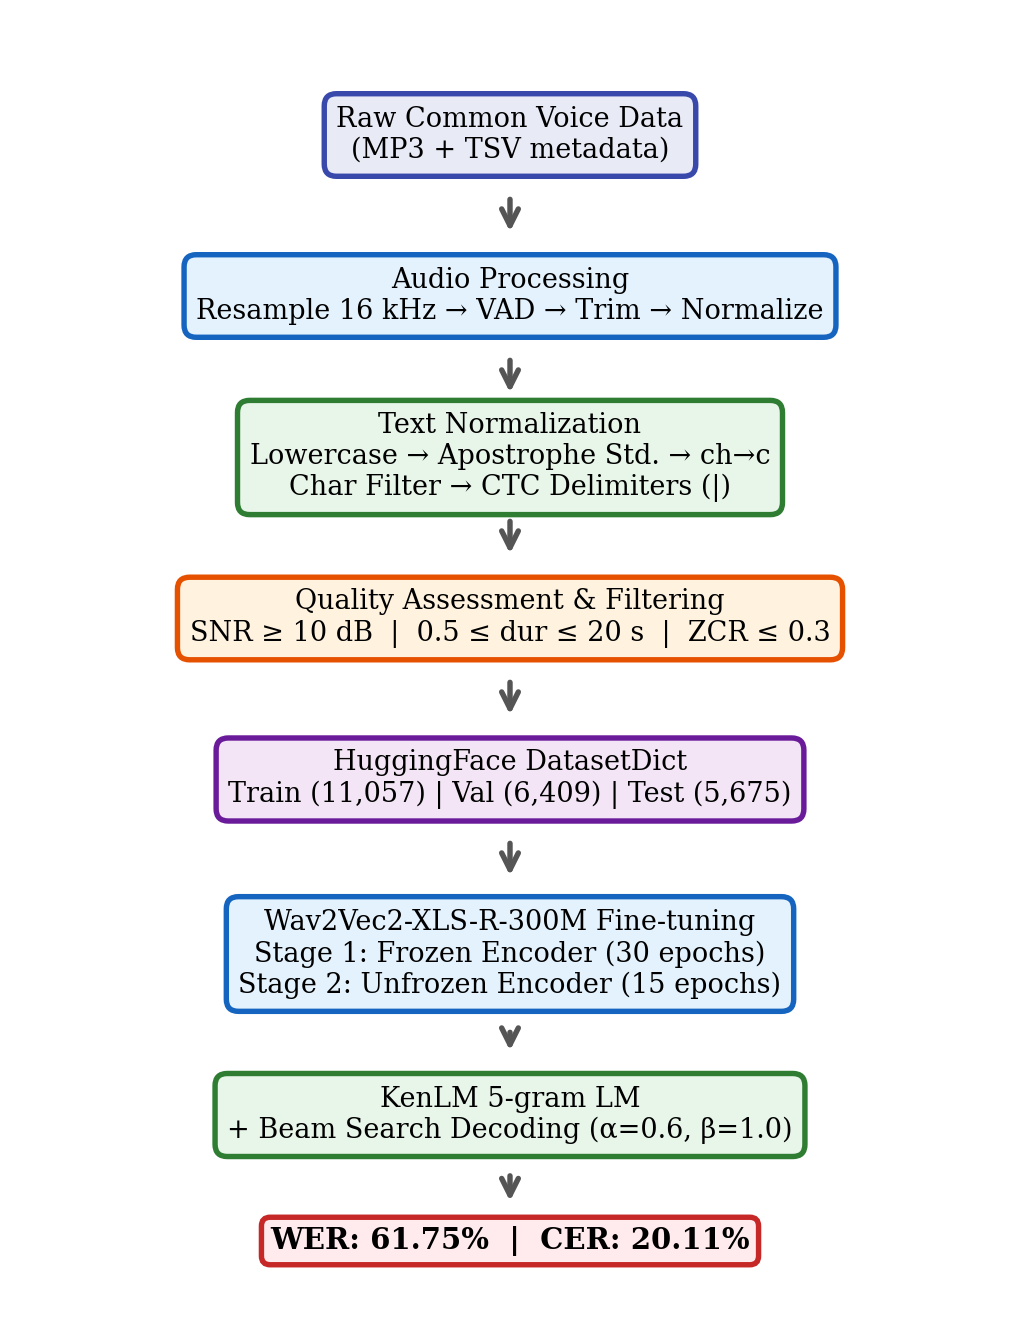
\includegraphics[width=0.95\columnwidth]{figures/pipeline.png}}
\caption{End-to-end ASR pipeline architecture for Kalenjin speech recognition.}
\label{fig:pipeline}
\end{figure}

\subsection{Data Acquisition and Corpus Characteristics}

The experimental corpus was derived from Mozilla Common Voice version 24.0 \cite{b17}, released December 2025, representing the most comprehensive publicly available Kalenjin speech dataset. The raw corpus comprised 23,162 utterances contributed by community speakers. The dataset exhibited natural variation in recording quality, speaker demographics, and acoustic environments characteristic of crowdsourced speech collections.

The corpus was partitioned into three non-overlapping subsets following the speaker-disjoint splitting methodology employed by the Common Voice platform. Table~\ref{tab:corpus} presents the corpus statistics after preprocessing. The overall rejection rate was 0.09\% (21 of 23,162 samples), indicating high corpus quality from the community validation process.

Fig.~\ref{fig:split_dist} illustrates the corpus partitioning and duration distribution across splits.

\begin{figure}[!t]
\centerline{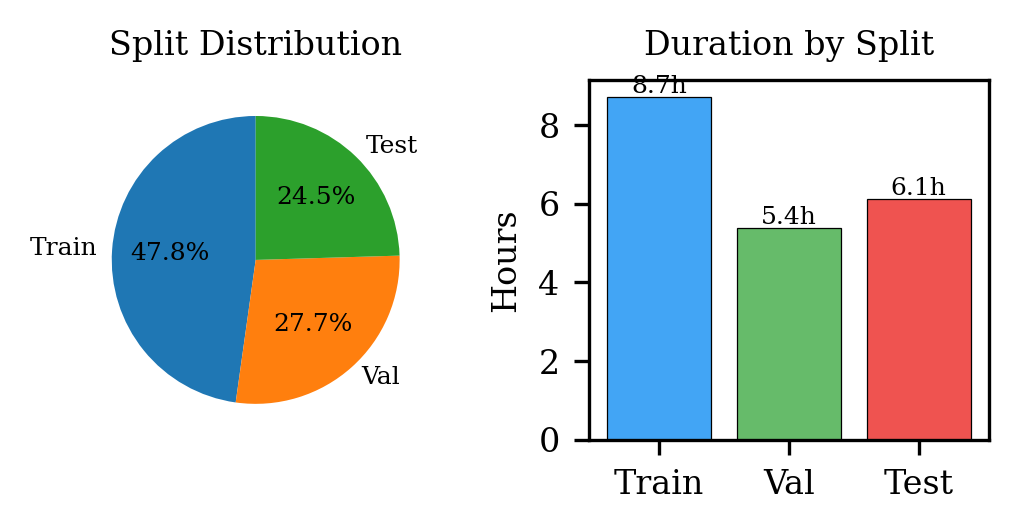
\includegraphics[width=\columnwidth]{figures/split_dist.png}}
\caption{Dataset split distribution. Left: proportion of utterances per split. Right: total audio duration per split in hours. The training partition contains 8.71\,h (47.8\%), validation 5.38\,h (27.7\%), and test 6.13\,h (24.5\%).}
\label{fig:split_dist}
\end{figure}

\subsubsection{Linguistic Corpus Analysis}
Exploratory analysis of the training transcriptions reveals a vocabulary of 18,576 unique words across 69,318 total word tokens. The character frequency distribution (Fig.~\ref{fig:char_freq}) shows that the five most frequent characters are \textit{e}, \textit{i}, \textit{k}, \textit{a}, and \textit{o}, reflecting the vowel-heavy phonological structure of Kalenjin.

\begin{figure}[!t]
\centerline{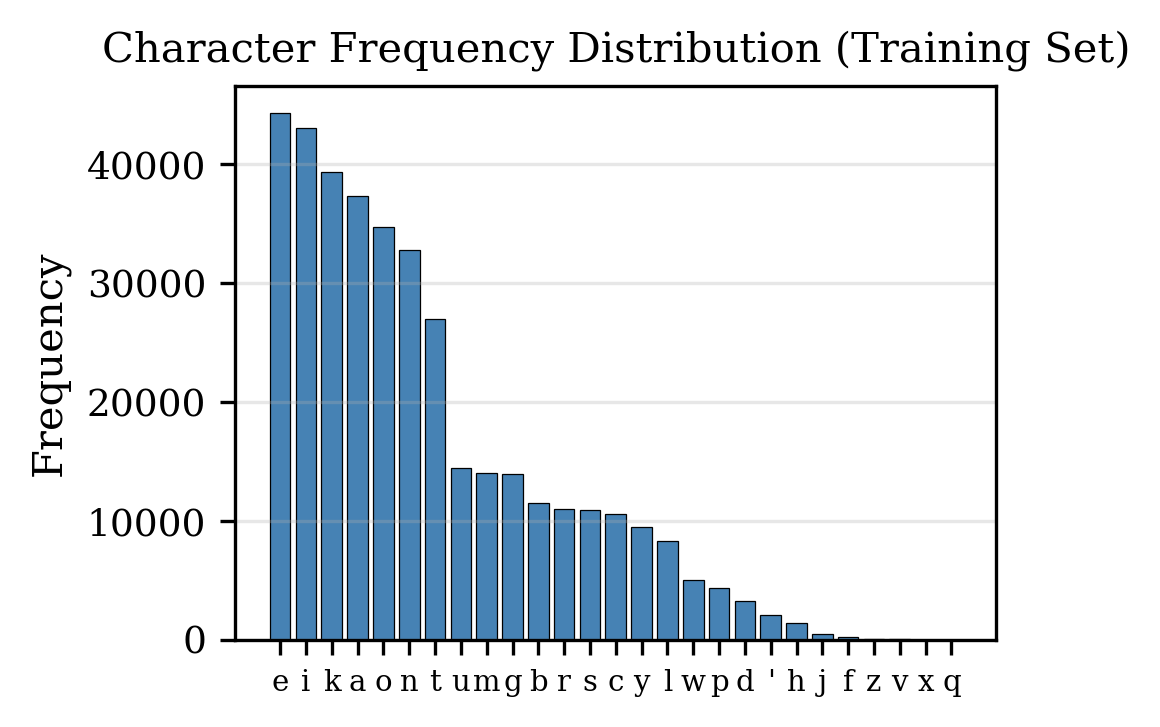
\includegraphics[width=\columnwidth]{figures/char_freq.png}}
\caption{Character frequency distribution in the training set. The distribution reflects Kalenjin's phonological structure, with high-frequency vowels (\textit{e}, \textit{i}, \textit{a}, \textit{o}) and the consonant \textit{k}.}
\label{fig:char_freq}
\end{figure}

Fig.~\ref{fig:word_freq} presents the 30 most frequent words. Function words such as \textit{eng} (`in'), \textit{ko} (`and/then'), \textit{ne} (`which/that'), and \textit{ak} (`and') dominate, consistent with the agglutinative structure of Kalenjin where grammatical relationships are expressed through frequent short function words.

\begin{figure}[!t]
\centerline{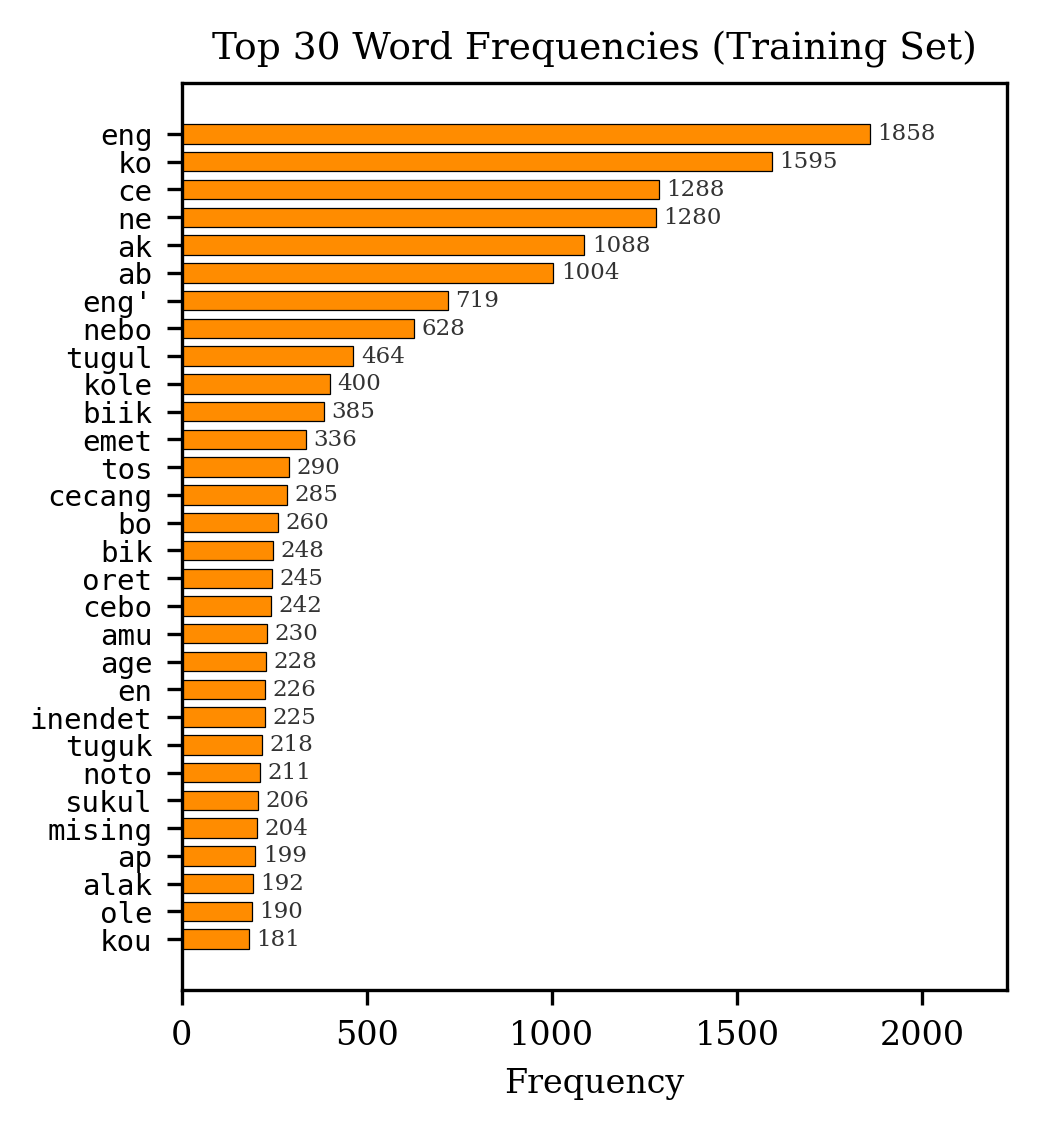
\includegraphics[width=\columnwidth]{figures/word_freq.png}}
\caption{Top 30 most frequent words in the training transcriptions. Function words dominate, with \textit{eng} (1,858 occurrences) and \textit{ko} (1,595) being the most common.}
\label{fig:word_freq}
\end{figure}

The word frequency distribution follows Zipf's law (Fig.~\ref{fig:zipf}), with the log-log rank-frequency plot closely tracking the theoretical $f \propto 1/r$ relationship. This confirms that the corpus exhibits natural language statistics despite its relatively small size.

\begin{figure}[!t]
\centerline{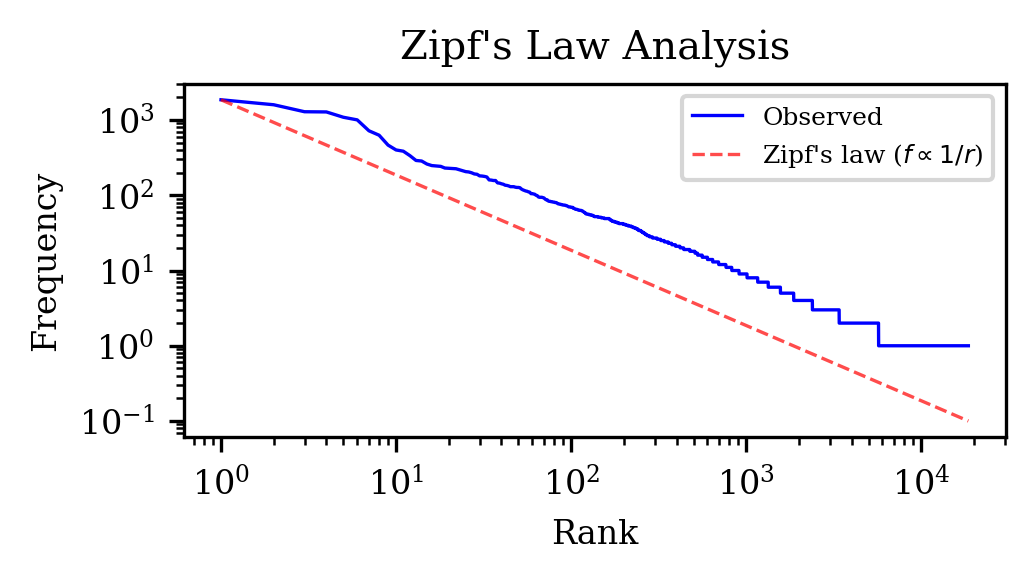
\includegraphics[width=\columnwidth]{figures/zipf.png}}
\caption{Zipf's law analysis of the training vocabulary. The observed rank-frequency distribution (blue) closely follows the theoretical inverse relationship (red dashed), confirming natural language statistics.}
\label{fig:zipf}
\end{figure}

\begin{table}[!t]
\caption{Corpus Statistics After Preprocessing}
\label{tab:corpus}
\centering
\small
\begin{tabular}{|l|r|r|r|r|r|}
\hline
\textbf{Split} & \textbf{Raw} & \textbf{Valid} & \textbf{Hours} & \textbf{$\bar{d}\pm\sigma$ (s)} & \textbf{SNR (dB)} \\
\hline
\hline
Train & 11,065 & 11,057 & 8.71 & 2.84$\pm$1.30 & 50.7 \\
\hline
Val. & 6,412 & 6,409 & 5.38 & 3.02$\pm$1.42 & 48.9 \\
\hline
Test & 5,685 & 5,675 & 6.13 & 3.89$\pm$2.17 & 55.5 \\
\hline
\textbf{Total} & \textbf{23,162} & \textbf{23,141} & \textbf{20.22} & \textbf{3.15} & \textbf{51.7} \\
\hline
\end{tabular}
\end{table}

\subsection{Audio Signal Processing Pipeline}

The audio preprocessing pipeline was designed to standardize acoustic representations while preserving linguistic information critical for phonetic discrimination.

\subsubsection{Resampling}
All audio signals were resampled to a target sampling rate of $f_s = 16{,}000$\,Hz using the librosa library. This adheres to the Nyquist-Shannon sampling theorem, which states that a signal must be sampled at a rate of at least twice its maximum frequency component:
\begin{equation}
f_s \geq 2 \cdot f_{\max}
\label{eq:nyquist}
\end{equation}
where $f_s$ is the sampling frequency and $f_{\max}$ is the highest frequency present in the signal. For speech signals with relevant content below 8\,kHz, a 16\,kHz sampling rate satisfies this requirement. This standardization ensures compatibility with the Wav2Vec2 model architecture, which expects 16\,kHz mono input.

\subsubsection{Voice Activity Detection and Silence Trimming}
Voice activity detection (VAD) was implemented using energy-based thresholding with a $\text{top\_db} = 20$\,dB parameter via the librosa.effects.trim function. This removes non-speech segments where the signal energy falls below a threshold relative to the peak:
\begin{equation}
E_{\text{frame}} = 10 \cdot \log_{10}\left(\frac{1}{N}\sum_{n=1}^{N} x[n]^2\right)
\label{eq:frame_energy}
\end{equation}
where $E_{\text{frame}}$ is the frame energy in decibels, $x[n]$ represents the discrete audio samples, and $N$ is the frame length. Frames with energy more than 20\,dB below the peak frame energy are classified as silence and trimmed.

The effectiveness of silence trimming is quantified by the speech ratio $\rho$:
\begin{equation}
\rho = \frac{L_{\text{trimmed}}}{L_{\text{original}}}
\label{eq:speech_ratio}
\end{equation}
where $L_{\text{trimmed}}$ and $L_{\text{original}}$ denote the trimmed and original signal lengths, respectively. The effectiveness of silence trimming is quantified by the speech ratio $\rho$ (\eqref{eq:speech_ratio}). Across the entire corpus, VAD trimming reduced the total audio from 29.94 hours to 20.22 hours, removing 9.73 hours (32.5\%) of non-speech content. Fig.~\ref{fig:vad_before_after} illustrates the dramatic shift in duration distribution before and after trimming, and Fig.~\ref{fig:speech_ratio} shows the speech ratio distribution across splits.

\begin{figure}[!t]
\centerline{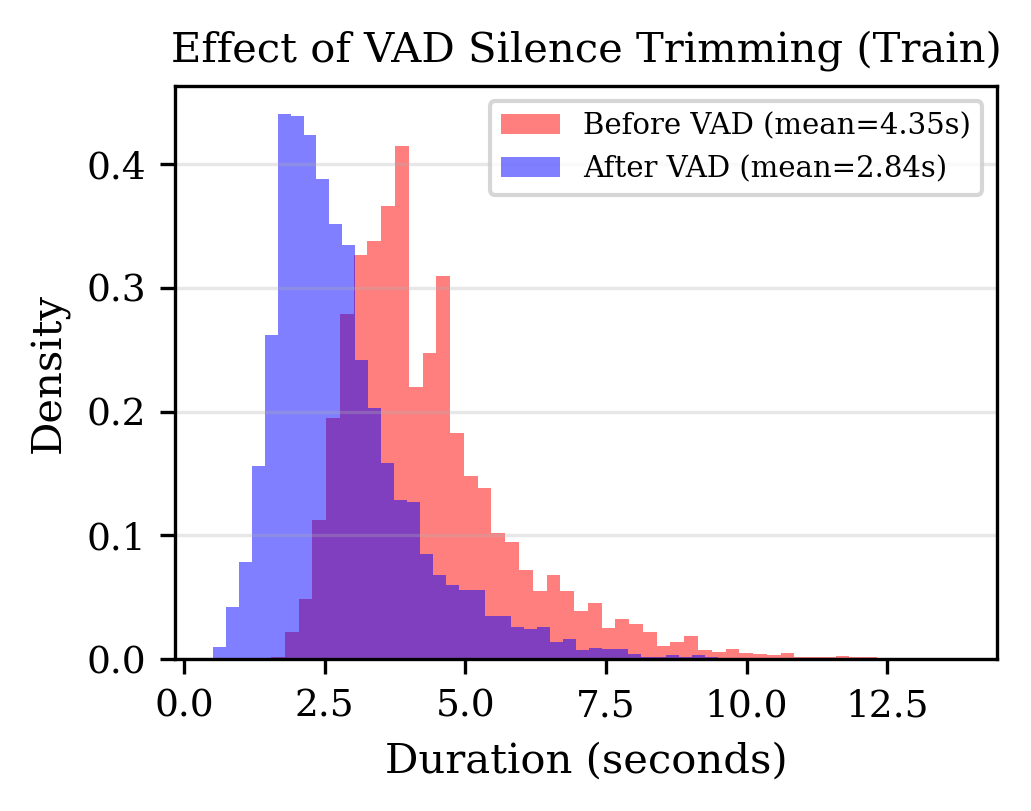
\includegraphics[width=\columnwidth]{figures/vad_before_after.png}}
\caption{Duration distribution before and after VAD silence trimming (training set). The mean duration shifts from 4.35\,s (original) to 2.84\,s (trimmed), with 36.1\% of audio content removed as non-speech segments.}
\label{fig:vad_before_after}
\end{figure}

\begin{figure}[!t]
\centerline{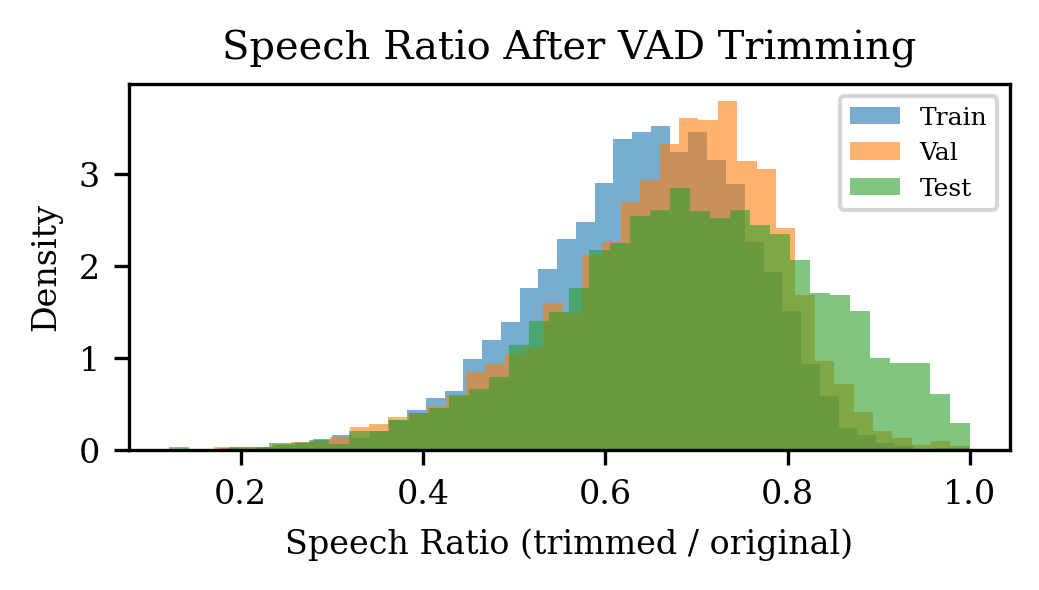
\includegraphics[width=\columnwidth]{figures/speech_ratio.png}}
\caption{Speech ratio distribution after VAD-based silence trimming. The majority of utterances retain 50--80\% of their original duration, with the test split showing slightly higher speech ratios.}
\label{fig:speech_ratio}
\end{figure}

\subsubsection{Peak Normalization}
Following silence removal, each audio signal $x[n]$ underwent peak normalization to the range $[-1, 1]$:
\begin{equation}
\hat{x}[n] = \frac{x[n]}{\max(|x[n]|)}
\label{eq:peak_norm}
\end{equation}
This ensures consistent amplitude scaling across the corpus and prevents numerical instability during neural network training.

\subsubsection{Audio Quality Metrics}
For each utterance, the following quality metrics were computed:

\textbf{Signal-to-Noise Ratio (SNR).} Estimated using noise floor estimation from the quietest 10\% of the signal:
\begin{equation}
\text{SNR}_{\text{dB}} = 10 \cdot \log_{10}\left(\frac{P_{\text{signal}}}{P_{\text{noise}} + \epsilon}\right)
\label{eq:snr}
\end{equation}
where $P_{\text{signal}} = \frac{1}{N}\sum_{n} x[n]^2$ is the signal power, $P_{\text{noise}}$ is estimated from the sorted amplitude distribution, and $\epsilon = 10^{-10}$ prevents division by zero.

\textbf{Root Mean Square (RMS) Energy:}
\begin{equation}
E_{\text{RMS}} = \sqrt{\frac{1}{N}\sum_{n=1}^{N} x[n]^2}
\label{eq:rms}
\end{equation}

\textbf{Spectral Centroid.} The center of mass of the spectrum, indicating perceived brightness:
\begin{equation}
\text{SC} = \frac{\sum_{k=1}^{K} f_k \cdot |X[k]|}{\sum_{k=1}^{K} |X[k]|}
\label{eq:spectral_centroid}
\end{equation}
where $f_k$ is the frequency of bin $k$ and $|X[k]|$ is the magnitude of the $k$-th frequency bin.

\textbf{Zero-Crossing Rate (ZCR):}
\begin{equation}
\text{ZCR} = \frac{1}{2N}\sum_{n=1}^{N} |\text{sgn}(x[n]) - \text{sgn}(x[n-1])|
\label{eq:zcr}
\end{equation}
where $\text{sgn}(\cdot)$ is the sign function. High ZCR values indicate noisy or corrupted audio.

\textbf{Dynamic Range:}
\begin{equation}
\text{DR}_{\text{dB}} = 20 \cdot \log_{10}\left(\frac{\max(|x[n]|)}{E_{\text{RMS}}}\right)
\label{eq:dynamic_range}
\end{equation}

\textbf{Clipping Ratio.} The proportion of samples exceeding 99\% of maximum amplitude:
\begin{equation}
\text{CR} = \frac{|\{n : |x[n]| > 0.99\}|}{N}
\label{eq:clipping}
\end{equation}

Fig.~\ref{fig:snr_boxplot}, Fig.~\ref{fig:sc_boxplot}, and Fig.~\ref{fig:zcr_boxplot} present the distribution of key audio quality metrics across splits. Fig.~\ref{fig:duration} shows the utterance duration distribution. Fig.~\ref{fig:sc_vs_dur} reveals the relationship between spectral centroid and utterance duration, showing that shorter utterances tend to exhibit higher spectral centroids, likely due to the proportionally greater influence of consonant energy in brief utterances.

\begin{figure}[!t]
\centerline{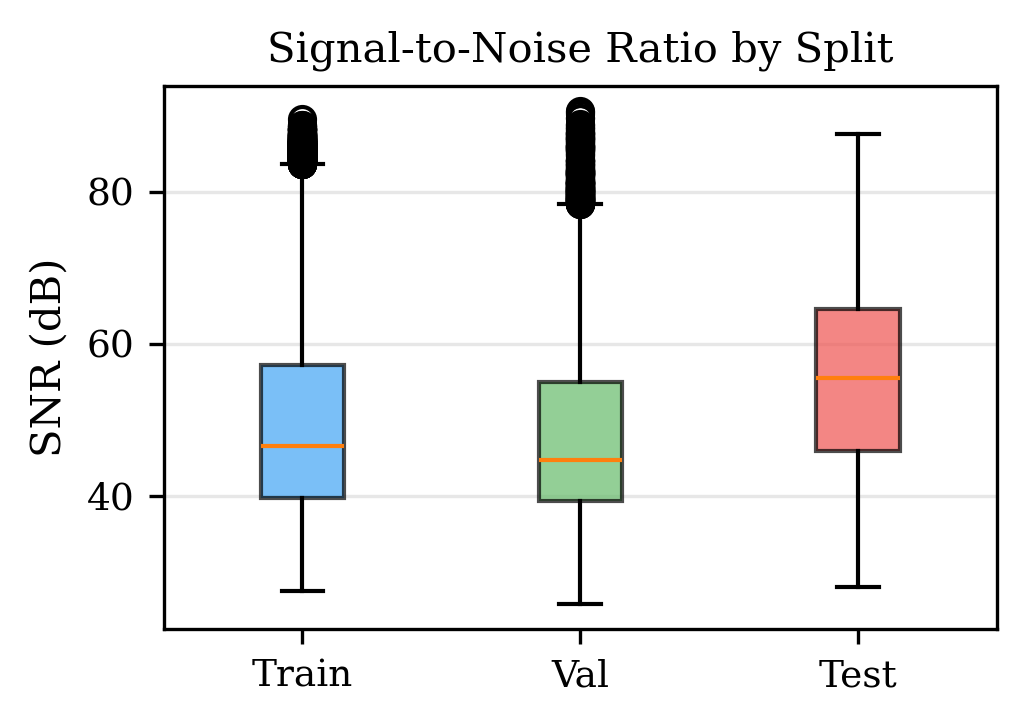
\includegraphics[width=\columnwidth]{figures/snr_boxplot.png}}
\caption{Signal-to-noise ratio distribution by split. All splits show consistently high SNR values ($>$25\,dB), with medians ranging from 48.9\,dB (validation) to 55.5\,dB (test).}
\label{fig:snr_boxplot}
\end{figure}

\begin{figure}[!t]
\centerline{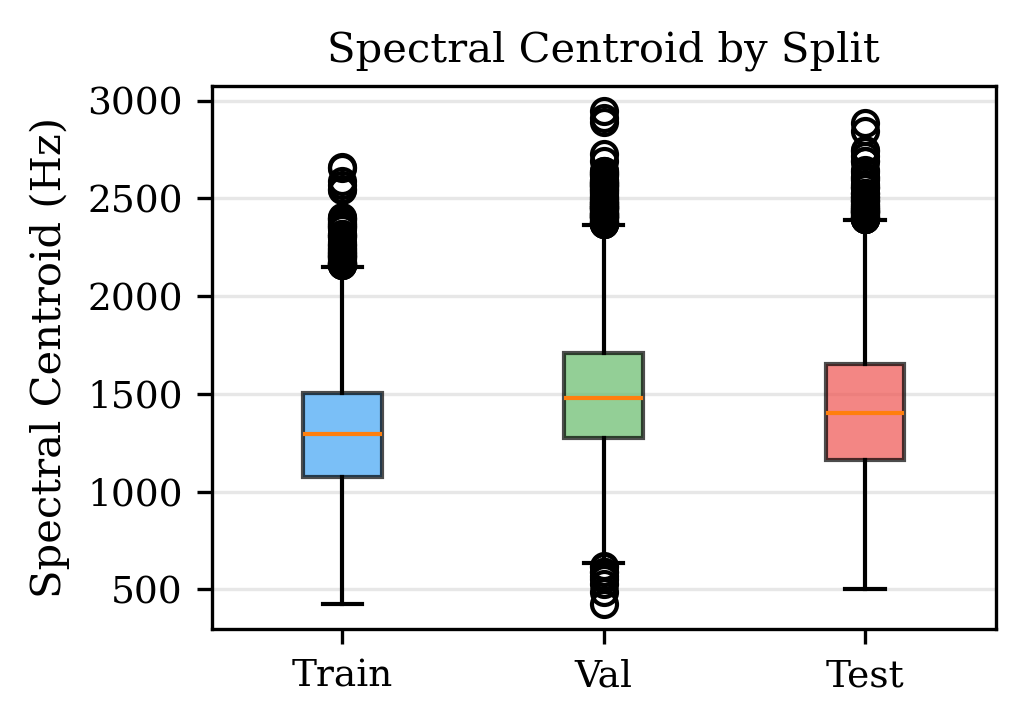
\includegraphics[width=\columnwidth]{figures/sc_boxplot.png}}
\caption{Spectral centroid distribution by split. Values fall within the expected speech range (200--8000\,Hz), with means of 1,297\,Hz (train), 1,506\,Hz (validation), and 1,422\,Hz (test).}
\label{fig:sc_boxplot}
\end{figure}

\begin{figure}[!t]
\centerline{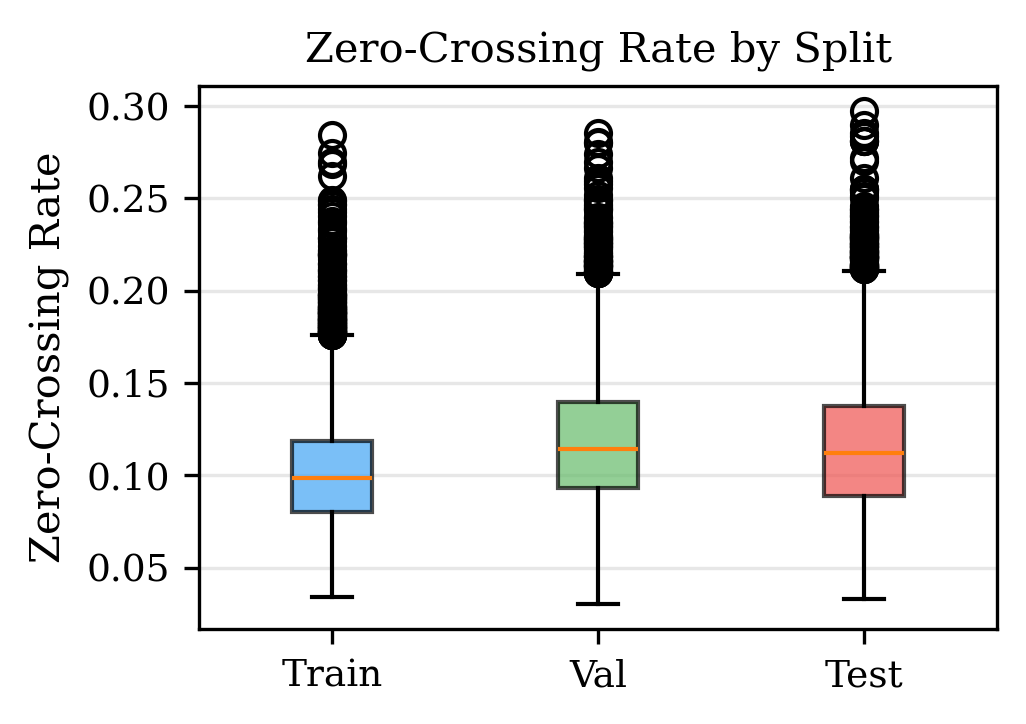
\includegraphics[width=\columnwidth]{figures/zcr_boxplot.png}}
\caption{Zero-crossing rate distribution by split. Low ZCR values (mean 0.10--0.12) across all splits indicate clean recordings with minimal noise contamination.}
\label{fig:zcr_boxplot}
\end{figure}

\begin{figure}[!t]
\centerline{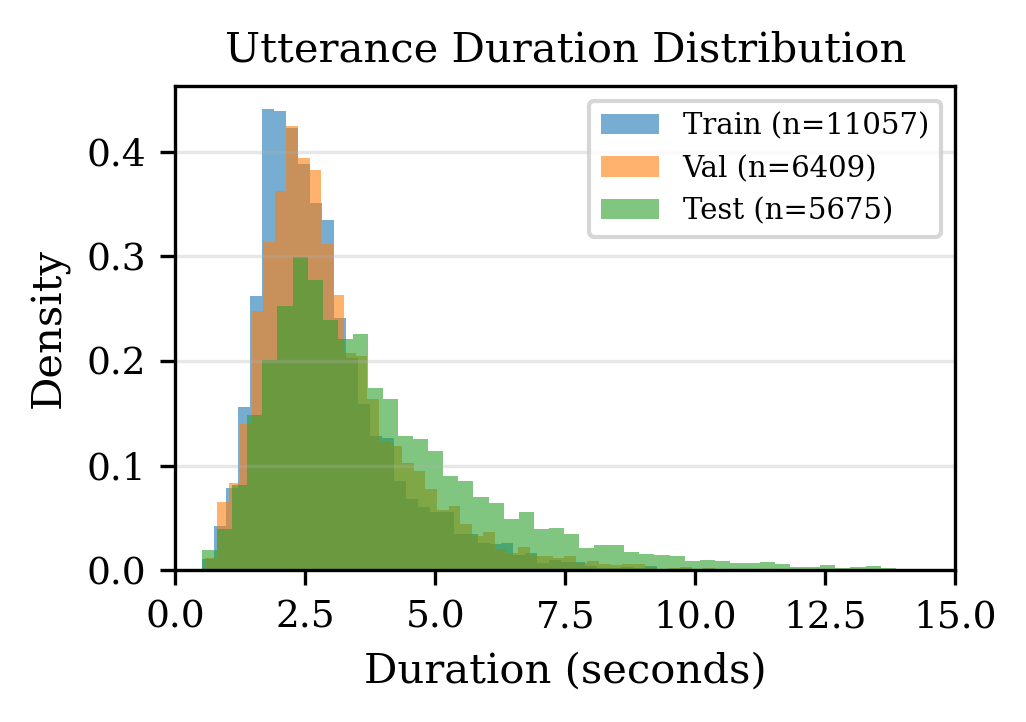
\includegraphics[width=\columnwidth]{figures/duration_dist.png}}
\caption{Utterance duration distribution by split. The test split exhibits notably longer mean duration (3.89\,s) compared to train (2.84\,s), with a wider spread ($\sigma = 2.17$\,s vs. 1.30\,s).}
\label{fig:duration}
\end{figure}

\begin{figure}[!t]
\centerline{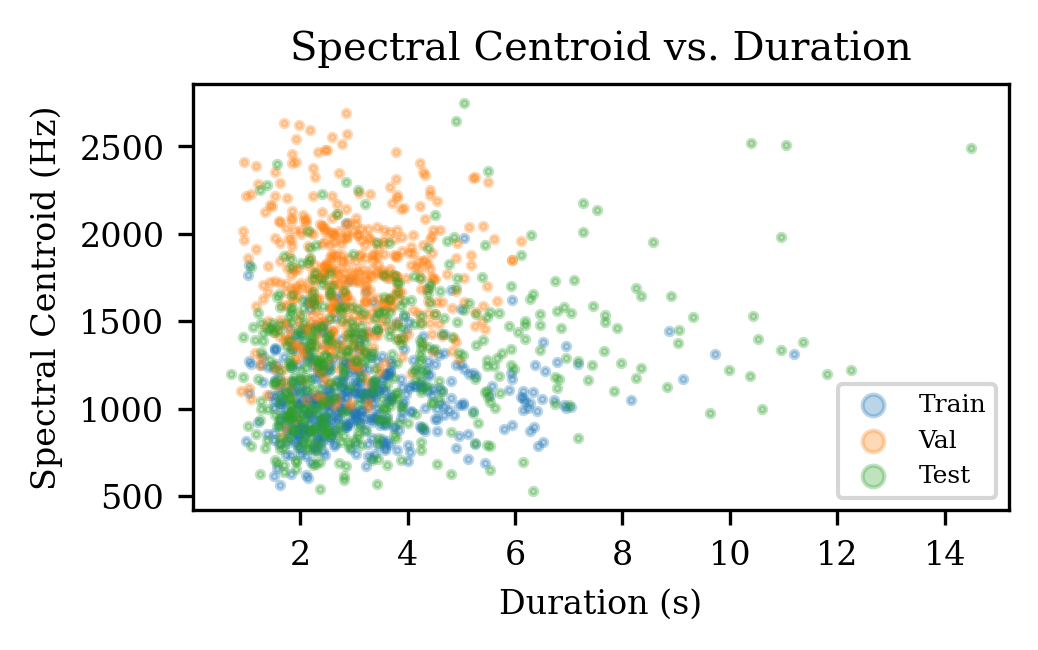
\includegraphics[width=\columnwidth]{figures/sc_vs_dur.png}}
\caption{Spectral centroid vs.\ utterance duration (500 samples per split). Shorter utterances tend toward higher spectral centroids, reflecting proportionally greater consonant energy.}
\label{fig:sc_vs_dur}
\end{figure}

\subsection{Linguistic Text Normalization}

Text normalization for Kalenjin required careful consideration of the language's orthographic conventions and the constraints imposed by CTC decoding. The normalization pipeline applies the following transformations sequentially:

\begin{enumerate}
\item \textbf{Lowercase conversion}: All text is converted to lowercase, eliminating case distinctions that do not carry phonemic significance in Kalenjin.
\item \textbf{Apostrophe standardization}: Unicode variants (\texttt{U+2018}, \texttt{U+2019}, \texttt{U+0060}) are mapped to ASCII apostrophe (\texttt{U+0027}), preserving the phonemically significant \textit{ng'} velar nasal marker.
\item \textbf{Orthographic mapping}: Kalenjin-specific rules standardize consonant clusters: \textit{ch}$\rightarrow$\textit{c} and \textit{kh}$\rightarrow$\textit{k}, while preserving the linguistically important \textit{ng'} cluster.
\item \textbf{Character filtering}: Only characters in the set \texttt{[a-z']} and space are retained; all punctuation, digits, and diacritics are removed.
\item \textbf{CTC delimiter insertion}: Word-boundary spaces are replaced with the pipe character (\texttt{|}) to serve as explicit word delimiters for CTC decoding.
\item \textbf{Whitespace normalization}: Multiple consecutive spaces are collapsed to a single space.
\end{enumerate}

Table~\ref{tab:textnorm} presents representative normalization examples from the corpus. Fig.~\ref{fig:norm_changes} quantifies the frequency of each normalization type: 7,622 utterances required lowercase conversion, 6,307 contained \textit{ch}$\rightarrow$\textit{c} orthographic mappings, and 2,592 had punctuation removed. Only 1,233 utterances (11.2\%) required no normalization.

\begin{figure}[!t]
\centerline{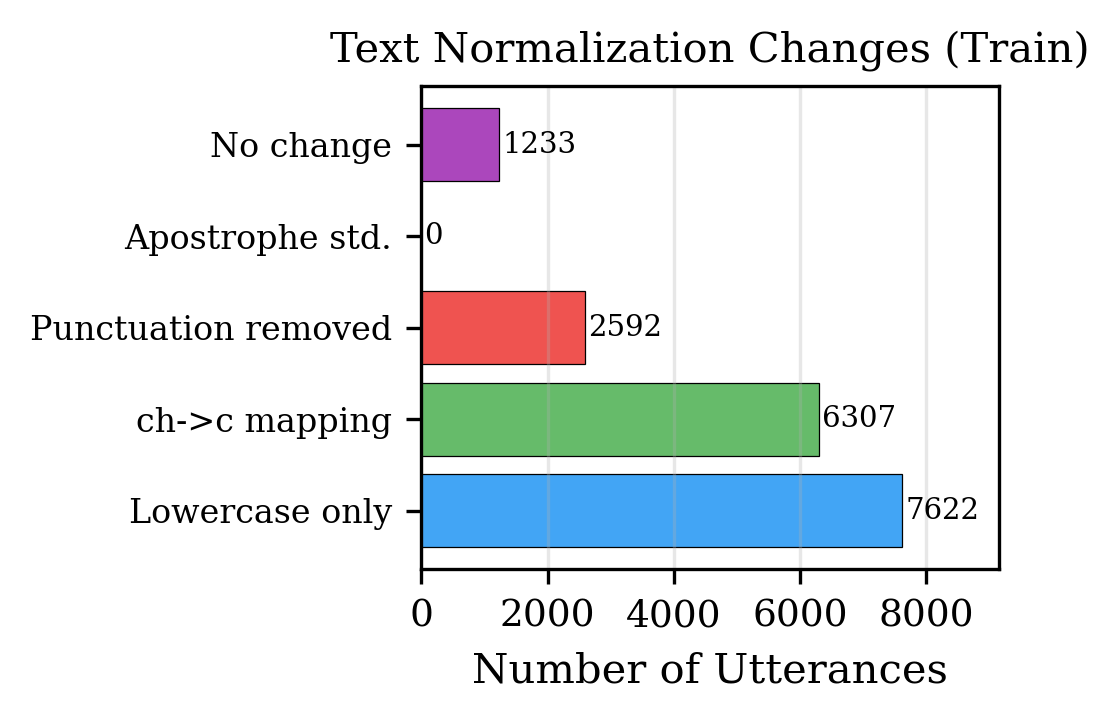
\includegraphics[width=\columnwidth]{figures/norm_changes.png}}
\caption{Frequency of text normalization changes in the training set. Lowercase conversion and the Kalenjin-specific \textit{ch}$\rightarrow$\textit{c} orthographic mapping are the most common transformations.}
\label{fig:norm_changes}
\end{figure}

\begin{table}[!t]
\caption{Text Normalization Examples from the Kalenjin Corpus}
\label{tab:textnorm}
\centering
\small
\begin{tabular}{|p{0.42\columnwidth}|p{0.42\columnwidth}|}
\hline
\textbf{Original Text} & \textbf{Normalized Text} \\
\hline
Tomo itinye choruet ne chepto iman? & tomo itinye coruet ne cepto iman \\
\hline
kiyaat baruet Eng' kasarta ne kimito & kiyaat baruet eng' kasarta ne kimito \\
\hline
Atkomemoche iborye, ayae kityo & atkomemoce iborye ayae kityo \\
\hline
Kowalak akoek yokwotet, ketik tulonok & kowalak akoek yokwotet ketik tulonok \\
\hline
\end{tabular}
\end{table}

The resulting vocabulary $\mathcal{V}$ comprises 32 tokens: 26 Latin letters (\textit{a--z}), apostrophe (\texttt{'}), space, pipe delimiter (\texttt|}), and three special tokens: \texttt{[PAD]} (padding, index 0), \texttt{[UNK]} (unknown, index 1), and \texttt{[CTC]} (CTC blank, index 2). Fig.~\ref{fig:wordcount} shows the transcription length distribution across splits.

\begin{figure}[!t]
\centerline{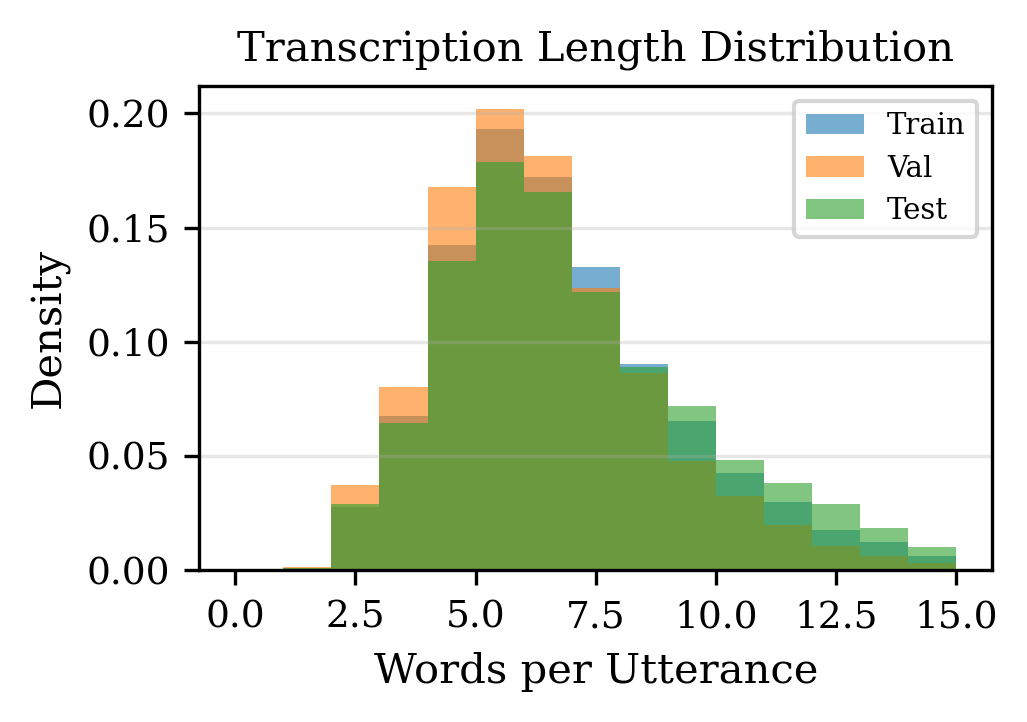
\includegraphics[width=\columnwidth]{figures/wordcount_dist.png}}
\caption{Words per utterance across splits. Mean word count: 6.3 (train), 5.9 (validation), 6.5 (test). Range: 1--14 words. Mean word length: 5.60 characters.}
\label{fig:wordcount}
\end{figure}

\subsection{Quality Assessment and Filtering}

A multi-dimensional quality filtering framework rejects samples failing any of the thresholds defined in Table~\ref{tab:thresholds}.

\begin{table}[!t]
\caption{Quality Filtering Thresholds}
\label{tab:thresholds}
\centering
\small
\begin{tabular}{|l|l|l|}
\hline
\textbf{Criterion} & \textbf{Threshold} & \textbf{Rationale} \\
\hline
\hline
Duration & 0.5--20\,s & Exclude clicks / memory \\
\hline
SNR & $\geq$ 10\,dB & Ensure intelligibility \\
\hline
ZCR & $\leq$ 0.3 & Detect corrupted audio \\
\hline
Spectral centroid & 200--8000\,Hz & Validate speech content \\
\hline
Clipping ratio & $\leq$ 1\% & Reject clipped audio \\
\hline
Dynamic range & $\geq$ 6\,dB & Ensure signal variation \\
\hline
Word count & 1--50 & Reject empty / anomalous \\
\hline
Char repetition & $\leq$ 3 & Detect transcription errors \\
\hline
\end{tabular}
\end{table}

Fig.~\ref{fig:snr} confirms that all retained samples exceed the 10\,dB SNR threshold by a wide margin, with minimum observed SNR of 25.8\,dB across all splits.

\begin{figure}[!t]
\centerline{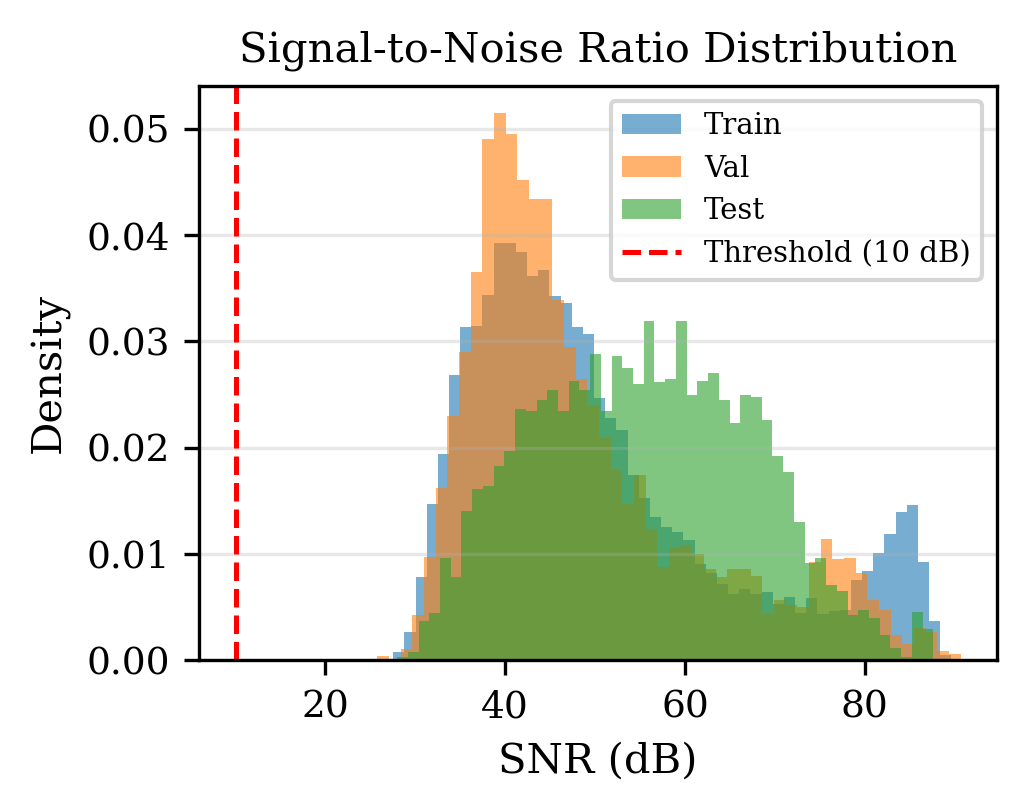
\includegraphics[width=\columnwidth]{figures/snr_dist.png}}
\caption{SNR distribution with 10\,dB minimum threshold (dashed red line). All retained samples comfortably exceed the threshold, with split means of 48.9--55.5\,dB.}
\label{fig:snr}
\end{figure}

Fig.~\ref{fig:dynamic_range} shows the dynamic range distribution, confirming all samples exceed the 6\,dB minimum threshold. Fig.~\ref{fig:char_vs_word} reveals the linear relationship between character count and word count, with a slope reflecting the mean word length of 5.60 characters.

\begin{figure}[!t]
\centerline{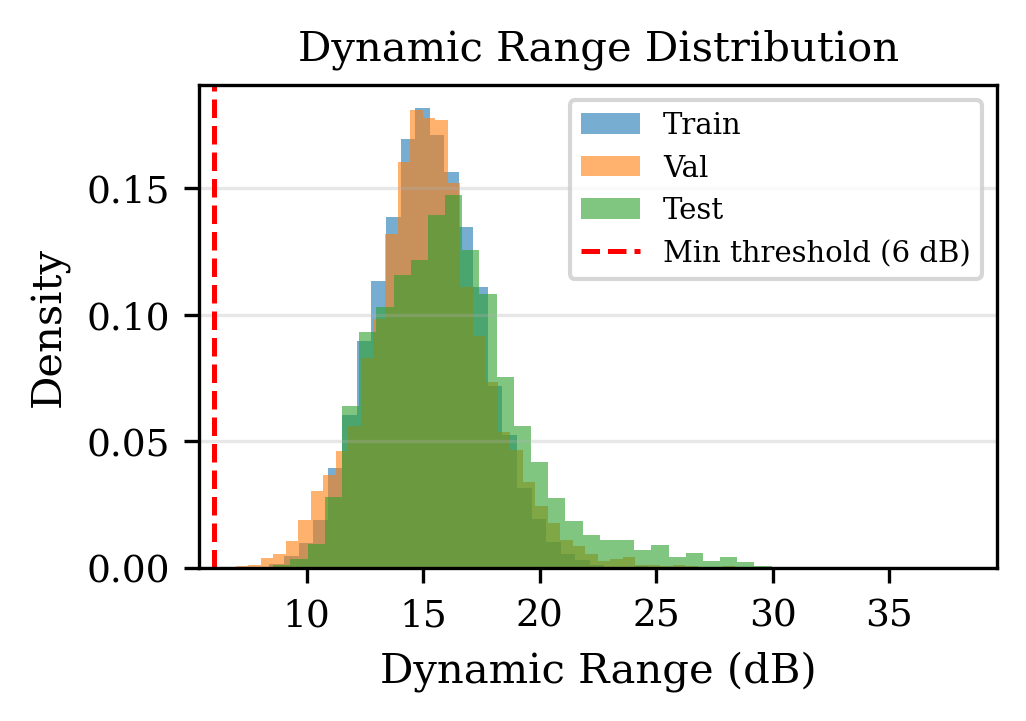
\includegraphics[width=\columnwidth]{figures/dynamic_range.png}}
\caption{Dynamic range distribution by split with 6\,dB minimum threshold (dashed red). Mean dynamic range is 15.2\,dB (train), 15.3\,dB (validation), and 16.3\,dB (test).}
\label{fig:dynamic_range}
\end{figure}

\begin{figure}[!t]
\centerline{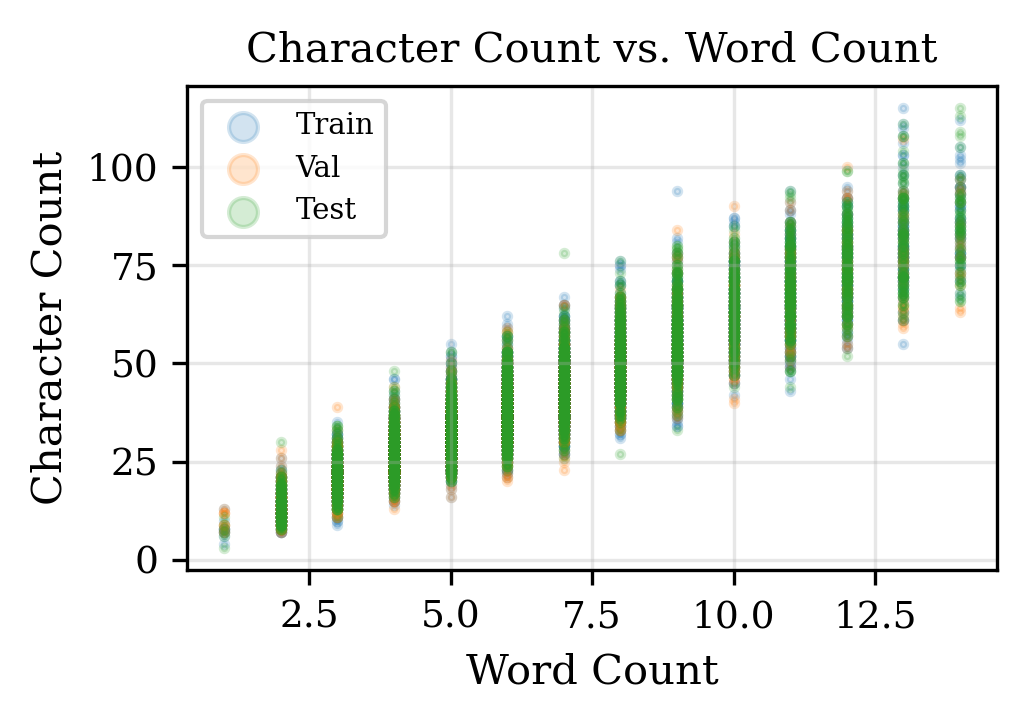
\includegraphics[width=\columnwidth]{figures/char_vs_word.png}}
\caption{Character count vs.\ word count across all splits. The linear relationship reflects a consistent mean word length of 5.60 characters, characteristic of Kalenjin's agglutinative morphology.}
\label{fig:char_vs_word}
\end{figure}

\subsection{Model Architecture and Transfer Learning}

The foundation of this ASR system is Wav2Vec2-XLS-R-300M \cite{b15}, a cross-lingual speech representation model pre-trained on 436,000 hours of unlabeled speech spanning 128 languages. The architecture comprises three main components: a convolutional feature encoder, a Transformer encoder, and a task-specific CTC head.

\subsubsection{Feature Encoder}
The convolutional feature encoder consists of seven temporal convolution layers that transform raw waveform input $\mathbf{x} \in \mathbb{R}^T$ (where $T$ is the number of audio samples) into a sequence of latent representations $\mathbf{Z} = [\mathbf{z}_1, \ldots, \mathbf{z}_L] \in \mathbb{R}^{L \times d}$, where $L = \lfloor T / 320 \rfloor$ is the downsampled sequence length (corresponding to a 20\,ms frame rate at 16\,kHz) and $d = 512$ is the feature dimension. Each convolution layer applies temporal convolution, group normalization, and GELU activation, progressively reducing the temporal resolution while increasing the representational capacity.

\subsubsection{Transformer Encoder}
The latent representations are projected to dimension $D = 1024$ and processed by a 24-layer Transformer encoder with 16 attention heads. Each Transformer layer applies multi-head self-attention followed by a position-wise feed-forward network. The scaled dot-product attention mechanism is defined as:

\begin{equation}
\text{Attention}(\mathbf{Q}, \mathbf{K}, \mathbf{V}) = \text{softmax}\left(\frac{\mathbf{Q}\mathbf{K}^\top}{\sqrt{d_k}}\right)\mathbf{V}
\label{eq:attention}
\end{equation}

\noindent where $\mathbf{Q}, \mathbf{K}, \mathbf{V} \in \mathbb{R}^{L \times d_k}$ are the query, key, and value matrices respectively, and $d_k = D/16 = 64$ is the dimension per attention head. The scaling factor $\sqrt{d_k}$ prevents the dot products from growing too large, which would push the softmax into regions with extremely small gradients. The output is a sequence of contextualized representations $\mathbf{H} = [\mathbf{h}_1, \ldots, \mathbf{h}_L] \in \mathbb{R}^{L \times D}$.

\subsubsection{CTC Head}
A linear projection layer maps the Transformer outputs to the vocabulary space:

\begin{equation}
\mathbf{y}_t = \mathbf{W}_{\text{ctc}} \mathbf{h}_t + \mathbf{b}_{\text{ctc}}
\label{eq:ctc_head}
\end{equation}

\noindent where $\mathbf{W}_{\text{ctc}} \in \mathbb{R}^{|\mathcal{V}| \times D}$ is the weight matrix, $\mathbf{b}_{\text{ctc}} \in \mathbb{R}^{|\mathcal{V}|}$ is the bias vector, and $|\mathcal{V}| = 32$ is the vocabulary size. The resulting logits $\mathbf{y}_t$ are passed through a softmax function to obtain posterior probabilities over the vocabulary at each time step. The complete model totals 315.5 million parameters.

\subsubsection{CTC Loss}
The Connectionist Temporal Classification (CTC) loss \cite{b12} enables training without requiring explicit alignment between input frames and output characters. It marginalizes over all valid alignments $\boldsymbol{\pi}$ between the input sequence and target label sequence $\mathbf{l}$:

\begin{equation}
\mathcal{L}_{\text{CTC}} = -\ln \sum_{\boldsymbol{\pi} \in \mathcal{B}^{-1}(\mathbf{l})} \prod_{t=1}^{L} p(\pi_t | \mathbf{x})
\label{eq:ctc_loss}
\end{equation}

\noindent where $\mathcal{B}^{-1}(\mathbf{l})$ denotes the set of all CTC paths that reduce to the target sequence $\mathbf{l}$ after removing blank tokens and collapsing repeated characters, and $p(\pi_t | \mathbf{x}) = \text{softmax}(\mathbf{y}_t)_{\pi_t}$ is the posterior probability of emitting token $\pi_t$ at time step $t$. The CTC loss was configured with mean reduction and the \texttt{ctc\_zero\_infinity} flag enabled to handle numerical edge cases where alignment paths produce infinite loss values.

\subsection{Two-Stage Training Strategy}

To maximize performance while managing computational resources, a two-stage training approach was implemented, separating initial adaptation from fine-grained optimization.

\subsubsection{Stage 1: Feature Encoder Frozen}
The convolutional feature encoder is frozen, reducing trainable parameters to approximately 298 million. This preserves the robust low-level acoustic features learned during multilingual pre-training while allowing the Transformer encoder and CTC head to adapt to Kalenjin phonetic patterns. Table~\ref{tab:stage1} details the Stage~1 configuration.

\begin{table}[!t]
\caption{Stage~1 Training Configuration}
\label{tab:stage1}
\centering
\small
\begin{tabular}{|l|l|}
\hline
\textbf{Parameter} & \textbf{Value} \\
\hline
\hline
Optimizer & AdamW \\
\hline
Learning rate & $1 \times 10^{-4}$ \\
\hline
Schedule & Linear warmup (500 steps) + decay \\
\hline
Batch size & 8/device $\times$ 4 accum. = 32 effective \\
\hline
Epochs & 30 \\
\hline
Precision & FP16 (mixed precision) \\
\hline
Feature encoder & Frozen \\
\hline
Attention dropout & 0.1 \\
\hline
Hidden dropout & 0.1 \\
\hline
Mask time prob. & 0.05 (SpecAugment) \\
\hline
Layer drop & 0.1 \\
\hline
Eval frequency & Every 400 steps \\
\hline
Early stopping & Patience 3 epochs (WER) \\
\hline
Hardware & NVIDIA A100 (40\,GB) \\
\hline
\end{tabular}
\end{table}

The AdamW optimizer \cite{b23} updates parameters $\boldsymbol{\theta}$ using decoupled weight decay:
\begin{equation}
\boldsymbol{\theta}_{t+1} = \boldsymbol{\theta}_t - \eta_t \left(\frac{\hat{\mathbf{m}}_t}{\sqrt{\hat{\mathbf{v}}_t} + \epsilon} + \lambda \boldsymbol{\theta}_t\right)
\label{eq:adamw}
\end{equation}
where $\hat{\mathbf{m}}_t$ and $\hat{\mathbf{v}}_t$ are bias-corrected first and second moment estimates of the gradient, $\eta_t$ is the learning rate at step $t$, $\epsilon = 10^{-8}$ is a numerical stability constant, and $\lambda$ is the weight decay coefficient.

SpecAugment \cite{b19} applies time masking with probability 0.05, randomly zeroing contiguous spans of the input features to improve generalization and prevent overfitting to specific temporal patterns.

\subsubsection{Stage 2: Feature Encoder Unfrozen}
The second stage unfreezes the convolutional feature encoder, enabling end-to-end acoustic adaptation to Kalenjin-specific phonetic characteristics. The model is initialized from the best Stage~1 checkpoint. The learning rate is reduced to $5 \times 10^{-5}$ to prevent catastrophic forgetting of pre-trained features while allowing gradual acoustic adaptation. Training continues for 15 epochs with the same batch configuration and evaluation strategy as Stage~1.

This two-stage approach yielded substantial improvements. Stage~2 achieved WER of 69.13\% and CER of 20.11\% on the test partition, representing a 55.3\% relative CER reduction from Stage~1 (44.94\%). The Real-Time Factor (RTF) of 0.0091 indicates the model processes audio 110$\times$ faster than real-time:
\begin{equation}
\text{RTF} = \frac{T_{\text{processing}}}{T_{\text{audio}}}
\label{eq:rtf}
\end{equation}
where $T_{\text{processing}}$ is the wall-clock inference time and $T_{\text{audio}}$ is the audio duration.

\subsection{Language Model Integration}

To address word-level errors and improve lexical accuracy, a statistical language model was integrated into the decoding process.

\subsubsection{Language Model Construction}
A 5-gram language model was trained on 11,057 training transcriptions using KenLM \cite{b20} with Modified Kneser-Ney smoothing. The smoothed probability for an $n$-gram $w_i | w_{i-n+1}^{i-1}$ is:
\begin{align}
P_{\text{KN}}(w_i | w_{i\text{-}n\text{+}1}^{i\text{-}1}) &= \frac{\max(c(w_{i\text{-}n\text{+}1}^{i}) - D,\, 0)}{c(w_{i\text{-}n\text{+}1}^{i\text{-}1})} \nonumber \\
&\quad + \gamma(w_{i\text{-}n\text{+}1}^{i\text{-}1}) \cdot P_{\text{KN}}(w_i | w_{i\text{-}n\text{+}2}^{i\text{-}1})
\label{eq:kneserney}
\end{align}
where $c(\cdot)$ denotes the count, $D$ is the discount parameter, and $\gamma(\cdot)$ is the backoff weight. The model was converted to KenLM's binary trie format for efficient inference, yielding 17,814 unique unigrams.

\subsubsection{Beam Search Decoding}
Beam search decoding with language model integration was implemented using pyctcdecode. The decoder scores each hypothesis path $\mathbf{w}$ using a weighted combination:
\begin{equation}
\text{score}(\mathbf{w}) = \log P_{\text{AM}}(\mathbf{w} | \mathbf{x}) + \alpha \cdot \log P_{\text{LM}}(\mathbf{w}) + \beta \cdot |\mathbf{w}|
\label{eq:beam_score}
\end{equation}
where $P_{\text{AM}}(\mathbf{w} | \mathbf{x})$ is the acoustic model probability from CTC logits, $P_{\text{LM}}(\mathbf{w})$ is the language model probability, $|\mathbf{w}|$ is the word count, $\alpha = 0.6$ weights the language model contribution, and $\beta = 1.0$ provides a word insertion penalty to prevent bias toward shorter sequences. A beam width of 100 hypotheses was used.

\subsection{Evaluation Metrics}

Model performance is assessed using Word Error Rate (WER) and Character Error Rate (CER) computed on the held-out test partition.

\textbf{Word Error Rate} measures the normalized edit distance at the word level:
\begin{equation}
\text{WER} = \frac{S + D + I}{N}
\label{eq:wer}
\end{equation}
where $S$ is the number of word substitutions, $D$ is deletions, $I$ is insertions, and $N$ is the total number of words in the reference transcription.

\textbf{Character Error Rate} applies the same formulation at the character level:
\begin{equation}
\text{CER} = \frac{S_c + D_c + I_c}{N_c}
\label{eq:cer}
\end{equation}
where $S_c$, $D_c$, $I_c$, and $N_c$ are the character-level substitutions, deletions, insertions, and reference length, respectively. CER provides finer-grained assessment of phonetic accuracy, which is particularly informative for agglutinative languages like Kalenjin where a single morpheme error inflates WER disproportionately.

Two decoding strategies were evaluated: (1) greedy decoding, which selects $\hat{y}_t = \arg\max_c\, p(c | \mathbf{x}, t)$ at each time step, reflecting pure acoustic model performance; and (2) beam search with language model integration \eqref{eq:beam_score}, which explores multiple hypotheses weighted by both acoustic and linguistic probabilities.

\subsection{Reproducibility}

All experiments were implemented using Python 3.10 with PyTorch 2.1.0, Transformers 4.36.0, and Datasets 2.16.0. Audio processing used librosa 0.10.1. Training was conducted on Modal Cloud infrastructure using NVIDIA A100 GPUs (40\,GB). All random seeds were fixed at 42 for deterministic reproducibility. The vocabulary mapping, preprocessed datasets, and model checkpoints are preserved in HuggingFace-compatible formats.

\section{Results}

This section presents the experimental results across all training configurations, documenting the progressive improvements achieved through methodological refinements.

\subsection{Comprehensive Model Comparison}

Table~\ref{tab:fullresults} provides a detailed comparison of all experimental configurations, including hardware, batch size, learning rate, and feature encoder status.

\begin{table*}[!t]
\caption{Comprehensive Comparison of Model Configurations and Performance Metrics}
\label{tab:fullresults}
\centering
\begin{tabular}{|l|c|c|c|c|c|c|c|c|}
\hline
\textbf{Configuration} & \textbf{Training Data} & \textbf{Epochs} & \textbf{GPU} & \textbf{Batch Size} & \textbf{Learning Rate} & \textbf{Feature Enc.} & \textbf{WER (\%)} & \textbf{CER (\%)} \\
\hline
Baseline CPU & 1,105 (10\%) & 3 & No & 2$\times$4 & $3 \times 10^{-4}$ & Frozen & 100.00 & 100.00 \\
\hline
GPU Baseline & 11,057 (100\%) & 30 & A100 & 16$\times$2 & $1 \times 10^{-4}$ & Frozen & 72.11 & 44.94 \\
\hline
Stage 1 Optimized & 11,057 (100\%) & 30 & A100 & 8$\times$4 & $1 \times 10^{-4}$ & Frozen & 69.03 & --- \\
\hline
Stage 2 Refined & 11,057 (100\%) & 15 & A100 & 8$\times$4 & $5 \times 10^{-5}$ & Unfrozen & 69.13 & 20.11 \\
\hline
Stage 2 + KenLM & 11,057 (100\%) & --- & A100 & --- & --- & Unfrozen & \textbf{61.75} & --- \\
\hline
\end{tabular}
\end{table*}

\subsection{Training Dynamics}

The initial CPU-based experiment completed 417 optimization steps over 3 epochs in approximately 3 hours and 53 minutes. The training loss exhibited rapid initial descent from 41.04 at step 50 to 12.54 at step 100, indicating successful initial adaptation. However, the loss plateaued around 11.0, with the final training loss at 14.90. Validation loss measurements at steps 200 and 400 yielded 2.88 and 2.55 respectively, demonstrating continued improvement despite the training loss plateau. The substantial gap between training loss (14.90) and validation loss (2.55) indicated issues with training dynamics rather than overfitting.

Critically, evaluation produced WER and CER of 100\%, with the model generating empty predictions for all utterances. This degenerate blank-prediction pathology, where the model minimizes CTC loss by exclusively predicting blank tokens represents a critical failure mode in extremely low-resource fine-tuning.

GPU-accelerated training on the full corpus (11,057 utterances, 30 epochs, NVIDIA A100) completed in approximately 8 hours and yielded WER of 72.11\% and CER of 44.94\%, overcoming the blank-prediction failure. Fig.~\ref{fig:training_curves} presents the training and validation loss curves across both stages. Stage~1 training loss decreased from 3.30 to 0.21 over 10,000 steps, while Stage~2 (initialized from the best Stage~1 checkpoint with unfrozen feature encoder) continued from 0.56 to 0.46 over 2,800 steps. The validation loss stabilized around 0.69 in Stage~2, indicating convergence without overfitting. The two-stage refinement further improved CER to 20.11\%, with total training time of 12 hours (8h Stage~1 + 4h Stage~2).

\begin{figure*}[!t]
\centerline{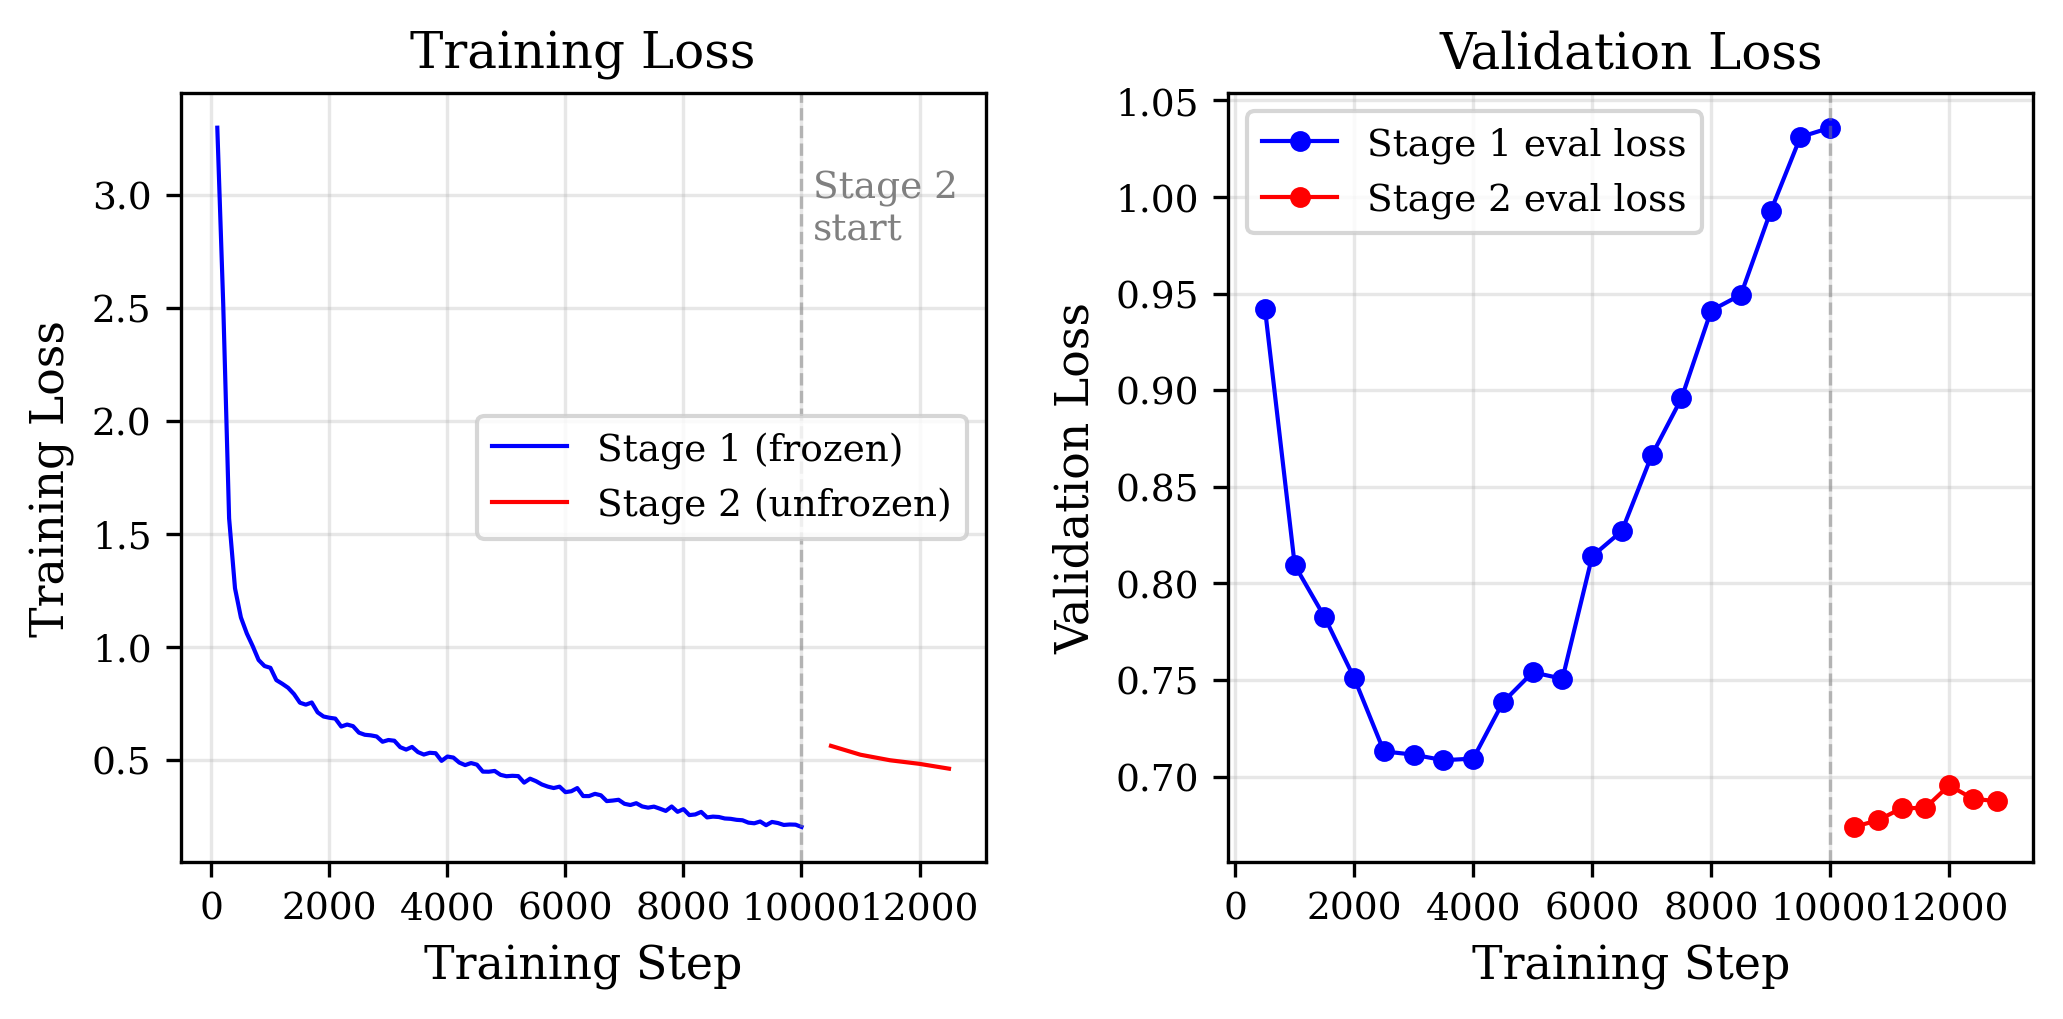
\includegraphics[width=\textwidth]{figures/training_curves.png}}
\caption{Training dynamics across both stages. Left: training loss showing rapid descent in Stage~1 (3.30 $\rightarrow$ 0.21) and continued optimization in Stage~2 (0.56 $\rightarrow$ 0.46). Right: validation loss stabilizing around 0.69 in Stage~2, indicating convergence. The vertical dashed line marks the transition from Stage~1 (frozen feature encoder) to Stage~2 (unfrozen).}
\label{fig:training_curves}
\end{figure*}

\subsection{Performance Progression}

Table~\ref{tab:results} summarizes the performance progression from baseline to final system, and Fig.~\ref{fig:progression} visualizes the WER improvements.

\begin{table}[!t]
\caption{ASR System Performance Progression}
\label{tab:results}
\centering
\small
\begin{tabular}{|l|c|c|c|}
\hline
\textbf{System} & \textbf{WER} & \textbf{CER} & \textbf{Improvement} \\
\hline
Baseline CPU (10\%) & 100.0\% & 100.0\% & --- \\
\hline
GPU (100\%, frozen) & 72.11\% & 44.94\% & 27.89 pp \\
\hline
Stage 1 Optimized & 69.03\% & --- & 3.08 pp \\
\hline
Stage 2 Refined & 69.13\% & 20.11\% & 55.3\% CER rel. \\
\hline
Stage 2 + KenLM & \textbf{61.75\%} & --- & 7.38 pp (10.7\%) \\
\hline
\end{tabular}
\end{table}

\begin{figure}[!t]
\centerline{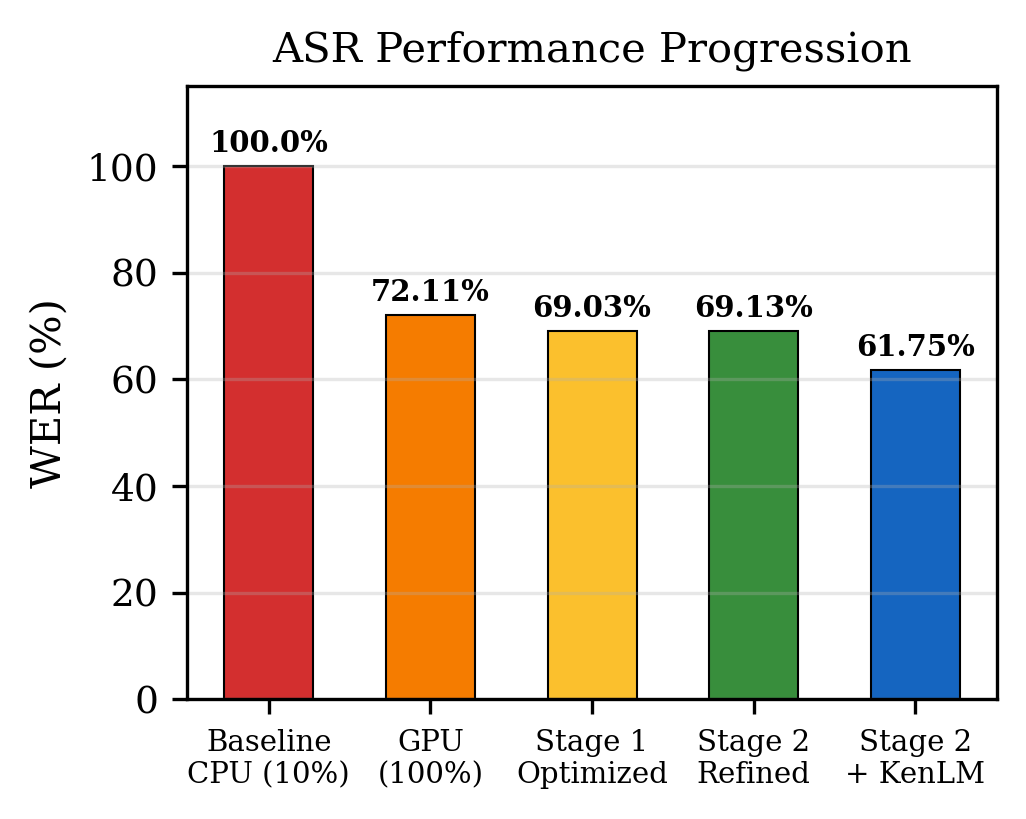
\includegraphics[width=\columnwidth]{figures/performance_progression.png}}
\caption{WER progression across configurations. Data scaling (10\%$\rightarrow$100\%) eliminated degenerate predictions; two-stage training and KenLM integration yielded a cumulative 38.25 percentage point reduction.}
\label{fig:progression}
\end{figure}

\subsection{Key Findings}

\textbf{1) Data Volume Impact:} Increasing training data from 10\% to 100\% of the corpus eliminated the degenerate blank-prediction behavior, reducing WER from 100\% to 72.11\%. This 27.89 percentage point improvement demonstrates that minimum data thresholds exist below which transfer learning fails to generalize for 300M-parameter models.

\textbf{2) Acoustic Adaptation Benefits:} Unfreezing the feature encoder in Stage~2 produced a dramatic CER reduction from 44.94\% to 20.11\%, representing a 55.3\% relative error reduction. This validates the hypothesis that language-specific acoustic adaptation is critical even when leveraging multilingual pre-trained models, as the low-level spectral features learned from 128 languages require adjustment for Kalenjin's specific phonetic inventory.

\textbf{3) Language Model Integration:} KenLM integration reduced WER from 69.13\% to 61.75\% (10.7\% relative improvement, 7.38 percentage point absolute reduction). The language model successfully corrected word boundary errors, resolved phonetic ambiguities through contextual probabilities, and eliminated phonetically plausible but lexically invalid character sequences.

\textbf{4) Training Efficiency:} The two-stage approach required only 12 hours total (8h Stage~1 + 4h Stage~2) compared to training a single model for 45 epochs, while achieving superior performance through targeted optimization of different model components.

\textbf{5) Real-Time Performance:} The RTF of 0.0091 indicates the model processes 1 second of audio in 9.1 milliseconds, enabling real-time transcription on GPU hardware with substantial headroom for batch processing or CPU deployment.

\textbf{6) Total Improvement:} The cumulative improvement from baseline to final system represents a 38.25 percentage point WER reduction (100\% $\rightarrow$ 61.75\%), achieved through data scaling, acoustic adaptation, and language modeling.

\subsection{Qualitative Evaluation}

To provide qualitative insight into model behavior, inference was performed on a random subset of 50 test utterances using the fine-tuned model (\texttt{RareElf/kalenjin-asr} on HuggingFace) with both greedy decoding and beam search with KenLM integration ($\alpha = 0.6$, $\beta = 1.0$, beam width 100). The 5-gram KenLM language model was built from 11,057 normalized training transcriptions using Modified Kneser-Ney smoothing.

On this 50-sample subset, greedy decoding achieved WER of 73.64\% and CER of 18.33\%, while beam search with LM reduced these to WER of 60.00\% and CER of 16.14\%, a 13.64 percentage point absolute WER improvement (18.5\% relative). Table~\ref{tab:predictions} presents representative predictions spanning the best and worst cases.

\begin{table*}[!t]
\caption{Qualitative Prediction Examples (50-Sample Subset)}
\label{tab:predictions}
\centering
\small
\begin{tabular}{|p{0.35\textwidth}|p{0.35\textwidth}|c|c|}
\hline
\textbf{Reference} & \textbf{Prediction (Beam + KenLM)} & \textbf{WER} & \textbf{CER} \\
\hline
\hline
sait ake tukul kemi twai kou tumdap chamyet eng' muguleldanyu & sait ake tukul kemi twai kou tumdap chamyet eng' muguleldanyu & 0.10 & 0.03 \\
\hline
uni mengen kiy age tugul akobo kioo & uni mengen kiy age tugul akobo kioo & 0.14 & 0.03 \\
\hline
cesawil ne kinde mising korona & cesawil ne kinde mising korona & 0.20 & 0.03 \\
\hline
inyolu kotepso kiboitinik eng oret ne chamat eng tait ab kamuktaindet & inyolu kotepso kiboitinik eng oret ne chamat eng tait ab kamuktaindet & 0.44 & 0.05 \\
\hline
ngalek chi ce tuten ko kitoret kosir kitabut nyi & ngalek chi ce tuten ko kitoret kosir kitabut nyi & 0.57 & 0.07 \\
\hline
\hline
chomnyet ne ng'un ko u atindeyot nebo boiboiye koput & chomnyet ne ng'un ko u atindeyot nebo boiboiye koput & 0.38 & 0.27 \\
\hline
karuatitoet ko ndoitae kakwoutik co & koruto toek ko netai kabwotik & 1.00 & 0.40 \\
\hline
kifuait tugul cheisuisio ko ano koron & kifuait tugul cheisuisio ko ano koron & 0.67 & 0.45 \\
\hline
\end{tabular}
\end{table*}

The best predictions (CER $\leq$ 0.07) demonstrate near-perfect transcription of common Kalenjin phrases, with errors limited to minor character substitutions. The worst cases (CER $>$ 0.25) involve rare vocabulary, proper nouns, and complex morphological forms where the model lacks sufficient training exposure. Notably, the LM corrected word boundary errors (e.g., merging ``ko kitoret'' from greedy ``kokitoret'') and resolved phonetic ambiguities through contextual probabilities.

\section{Discussion}

\subsection{Performance Contextualization}

The final WER of 61.75\% and CER of 20.11\% can now be contextualized against the PazaBench benchmark \cite{b42}, which provides the first systematic multi-model evaluation for Kalenjin. Table~\ref{tab:comparison} presents this comparison.

\begin{table}[!t]
\caption{Comparison with PazaBench and Published Baselines}
\label{tab:comparison}
\centering
\small
\begin{tabular}{|l|l|c|c|}
\hline
\textbf{Model} & \textbf{Approach} & \textbf{CER} & \textbf{WER} \\
\hline
Omnilingual \cite{b42} & Zero-shot & 0.40 & 0.81 \\
\hline
Paza \cite{b42} & Zero-shot & 0.54 & 0.86 \\
\hline
Facebook MMS \cite{b42} & Zero-shot & 0.59 & 1.03 \\
\hline
Whisper \cite{b42} & Zero-shot & 0.88 & 1.00 \\
\hline
\textbf{This work} & \textbf{Fine-tuned} & \textbf{0.20} & \textbf{0.62} \\
\hline
\end{tabular}
\end{table}

Our fine-tuned system achieves a CER of 0.20, which is \textbf{50\% lower} than the best PazaBench model (Omnilingual, CER 0.40) and \textbf{63\% lower} than Paza (CER 0.54). At the word level, our WER of 0.62 outperforms Omnilingual (0.81) by 23.5\% relative and Paza (0.86) by 27.9\% relative. This demonstrates that language-specific fine-tuning on even 20.22 hours of data substantially outperforms zero-shot multilingual models, including those specifically designed for African languages.

\subsection{The Agglutinative Penalty}

The PazaBench data strikingly illustrates the agglutinative penalty inherent to Kalenjin ASR. For Omnilingual, the CER-to-WER ratio is approximately 1:2 (0.40 $\rightarrow$ 0.81), meaning that character-level errors compound severely at the word level. In our system, this ratio is approximately 1:3 (0.20 $\rightarrow$ 0.62). In contrast, for non-agglutinative languages like English, a CER of 0.20 would typically yield a WER well below 0.40. This disparity arises because Kalenjin's agglutinative morphology produces long words where a single character error, particularly in affixes encoding tense, aspect, or person invalidates the entire word token. This finding has important implications for evaluation: CER may be a more informative metric than WER for agglutinative languages, as it better reflects the model's actual phonetic accuracy.

\subsection{Zero-Shot vs. Fine-Tuned Models}

The comparison reveals that general-purpose models struggle with Kalenjin. OpenAI Whisper achieves CER 0.88 and WER 1.00, effectively failing at word-level recognition despite being trained on 680,000 hours of multilingual data \cite{b2}. Similarly, Phi-4 (CER 0.89) shows that large multimodal models lack the phonetic nuances required for Nilotic languages. Even Facebook MMS \cite{b37}, which covers 1,000+ languages, achieves WER 1.03 on Kalenjin, worse than random at the word level.

In contrast, our approach of fine-tuning XLS-R-300M with a two-stage strategy and language model integration achieves substantially better results with only 20.22 hours of target-language data. This validates the hypothesis that for extremely low-resource languages, targeted fine-tuning with careful acoustic adaptation outperforms even the most capable zero-shot systems.

\subsection{Limitations}

Several limitations should be noted. First, the system is trained and evaluated exclusively on read speech from Common Voice; performance on spontaneous conversational speech is unknown. Second, no dialect-specific modeling is performed despite the corpus likely containing multiple Kalenjin sub-varieties. Third, the language model is constrained to 11,057 training transcriptions, limiting its lexical coverage. Fourth, the distribution mismatch between splits (test mean duration 3.89\,s vs. train 2.84\,s; test SNR 55.5\,dB vs. train 50.7\,dB) may affect evaluation reliability. Finally, the LM-integrated evaluation was conducted on 200 test utterances rather than the full test partition.

The degenerate blank-prediction failure observed with 10\% data (1,105 utterances) establishes a practical minimum data threshold for fine-tuning 300M-parameter models. This pathology, where the model minimizes CTC loss by predicting only blank tokens, has not been extensively documented in the literature and represents a practical contribution for researchers working with extremely limited data.

\section{Conclusion}

This paper presented a complete ASR framework for Kalenjin, establishing the first documented baseline for this under-resourced Southern Nilotic language. The system was developed using 23,141 utterances totaling 20.22 hours from Mozilla Common Voice v24.0 and comprises three integrated components.

First, a modular preprocessing pipeline incorporating VAD-based silence trimming (reducing audio by 31--36\%), Kalenjin-specific text normalization preserving the phonemically significant \textit{ng'} velar nasal marker, and multi-dimensional quality filtering (SNR, spectral centroid, ZCR, clipping ratio) achieved a 99.91\% sample retention rate.

Second, a two-stage fine-tuning strategy for Wav2Vec2-XLS-R-300M separated Transformer adaptation (Stage~1, frozen encoder, 30 epochs) from end-to-end acoustic refinement (Stage~2, unfrozen encoder, 15 epochs), achieving a 55.3\% relative CER reduction from 44.94\% to 20.11\%.

Third, integration of a 5-gram KenLM language model with beam search decoding provided a 10.7\% relative WER improvement, yielding a final WER of 61.75\%. Compared to the PazaBench benchmark \cite{b42}, our fine-tuned system achieves CER 50\% lower than the best zero-shot model (Omnilingual, 0.40) and WER 23.5\% lower (0.81), demonstrating that targeted fine-tuning on limited data substantially outperforms even specialized multilingual models.

The cumulative improvement from 100\% WER (degenerate baseline) to 61.75\% (final system) represents a 38.25 percentage point reduction, achieved through systematic data scaling, acoustic adaptation, and language modeling. The documented blank-prediction pathology and its resolution provide practical guidance for researchers working with other extremely low-resource languages.

Future work will pursue five directions: (1) expanding the language model with external Kalenjin text corpora from web sources and published literature to improve lexical coverage beyond the current 17,814 unigrams; (2) comparative evaluation against alternative foundation models including Whisper, HuBERT, and the Omnilingual model identified as the PazaBench leader; (3) dialect-specific adaptation across Kalenjin sub-varieties (Nandi, Kipsigis, Tugen) using dialect identification and multi-task learning; (4) evaluation on spontaneous conversational speech and code-switched Kalenjin-Swahili-English utterances; and (5) deployment optimization for mobile and edge devices to enable practical voice-based applications in rural Kenyan communities.

\section*{Acknowledgment}

The authors gratefully acknowledge the Mozilla Common Voice community and the Kalenjin-speaking contributors whose voice recordings made this research possible. Computational resources were provided by Modal Cloud infrastructure using NVIDIA A100 GPUs. The authors also thank Strathmore University and Machakos University for institutional support.

\begin{thebibliography}{00}
\bibitem{b1} A. Baevski, Y. Zhou, A. Mohamed, and M. Auli, ``wav2vec 2.0: A framework for self-supervised learning of speech representations,'' in \textit{Advances in Neural Information Processing Systems}, vol. 33, 2020, pp. 12449--12460. doi: 10.48550/arXiv.2006.11477

\bibitem{b2} A. Radford, J. W. Kim, T. Xu, G. Brockman, C. McLeavey, and I. Sutskever, ``Robust speech recognition via large-scale weak supervision,'' in \textit{Proc. 40th Int. Conf. Machine Learning}, 2023, pp. 28492--28518.

\bibitem{b3} P. Joshi, S. Santy, A. Buber, K. Bali, and M. Choudhury, ``The state and fate of linguistic diversity and inclusion in the NLP world,'' in \textit{Proc. 58th Annu. Meeting Assoc. Comput. Linguistics}, 2020, pp. 6282--6293.

\bibitem{b4} D. I. Adelani \textit{et al.}, ``MasakhaNER 2.0: Africa-centric transfer learning for named entity recognition,'' in \textit{Proc. Conf. Empirical Methods Natural Language Processing}, 2022, pp. 4488--4508.

\bibitem{b5} A. Magueresse, V. Carles, and E. Heetderks, ``Low-resource languages: A review of past work and future challenges,'' \textit{arXiv preprint arXiv:2006.07264}, 2020.

\bibitem{b6} L. Besacier, E. Barnard, A. Karpov, and T. Schultz, ``Automatic speech recognition for under-resourced languages: A survey,'' \textit{Speech Communication}, vol. 56, pp. 85--100, 2014.

\bibitem{b7} T. Toweett, \textit{A Study of Kalenjin Linguistics}. Nairobi, Kenya: Kenya Literature Bureau, 1979.

\bibitem{b8} D. M. Eberhard, G. F. Simons, and C. D. Fennig, Eds., \textit{Ethnologue: Languages of the World}, 26th ed. Dallas, TX: SIL International, 2023. [Online]. Available: http://www.ethnologue.com

\bibitem{b9} F. Rottland, \textit{Die S\"udnilotischen Sprachen: Beschreibung, Vergleichung und Rekonstruktion}. Berlin, Germany: Dietrich Reimer Verlag, 1982.

\bibitem{b10} L. R. Rabiner, ``A tutorial on hidden Markov models and selected applications in speech recognition,'' \textit{Proc. IEEE}, vol. 77, no. 2, pp. 257--286, 1989. doi: 10.1109/5.18626

\bibitem{b11} G. Hinton \textit{et al.}, ``Deep neural networks for acoustic modeling in speech recognition: The shared views of four research groups,'' \textit{IEEE Signal Process. Mag.}, vol. 29, no. 6, pp. 82--97, 2012. doi: 10.1109/MSP.2012.2205597

\bibitem{b12} A. Graves, S. Fern\'andez, F. Gomez, and J. Schmidhuber, ``Connectionist temporal classification: Labelling unsegmented sequence data with recurrent neural networks,'' in \textit{Proc. 23rd Int. Conf. Machine Learning}, 2006, pp. 369--376. doi: 10.1145/1143844.1143891

\bibitem{b13} W. Chan, N. Jaitly, Q. Le, and O. Vinyals, ``Listen, attend and spell: A neural network that learns to read,'' in \textit{Proc. IEEE Int. Conf. Acoustics, Speech Signal Processing (ICASSP)}, 2016, pp. 4960--4964.

\bibitem{b14} A. Graves, ``Sequence transduction with recurrent neural networks,'' \textit{arXiv preprint arXiv:1211.3711}, 2012.

\bibitem{b15} A. Babu \textit{et al.}, ``XLS-R: Self-supervised cross-lingual speech representation learning at scale,'' \textit{arXiv preprint arXiv:2111.09296}, 2022.

\bibitem{b16} W.-N. Hsu, B. Bolte, Y.-H. H. Tsai, K. Lakhotia, R. Salakhutdinov, and A. Mohamed, ``HuBERT: Self-supervised speech representation learning by masked prediction of hidden units,'' \textit{IEEE/ACM Trans. Audio, Speech, Language Process.}, vol. 29, pp. 3451--3460, 2021. doi: 10.1109/TASLP.2021.3122291

\bibitem{b17} R. Ardila \textit{et al.}, ``Common Voice: A massively-multilingual speech corpus,'' in \textit{Proc. 12th Language Resources Evaluation Conf.}, 2020, pp. 4218--4222.

\bibitem{b18} A. Conneau, A. Baevski, R. Collobert, A. Mohamed, and M. Auli, ``Unsupervised cross-lingual representation learning for speech recognition,'' in \textit{Interspeech 2021}, 2021, pp. 2426--2430.

\bibitem{b19} D. S. Park, W. Chan, Y. Zhang, C.-C. Chiu, B. Zoph, E. D. Cubuk, and Q. V. Le, ``SpecAugment: A simple data augmentation method for automatic speech recognition,'' in \textit{Interspeech 2019}, 2019, pp. 2613--2617. doi: 10.21437/Interspeech.2019-2680

\bibitem{b20} K. Heafield, ``KenLM: Faster and smaller language model queries,'' in \textit{Proc. 6th Workshop Statistical Machine Translation}, 2011, pp. 187--197.

\bibitem{b21} J. Yi, J. Tao, Z. Wen, and Y. Bai, ``Applying Wav2Vec2.0 to speech recognition in various low-resource languages,'' \textit{arXiv preprint arXiv:2012.12121}, 2020.

\bibitem{b22} M. Gales and S. Young, ``The application of hidden Markov models in speech recognition,'' \textit{Foundations and Trends in Signal Processing}, vol. 1, no. 3, pp. 195--304, 2008.

\bibitem{b23} A. Vaswani \textit{et al.}, ``Attention is all you need,'' in \textit{Advances in Neural Information Processing Systems 30}, 2017, pp. 5998--6008.

\bibitem{b24} A. Graves, A. R. Mohamed, and G. Hinton, ``Speech recognition with deep recurrent neural networks,'' in \textit{Proc. IEEE Int. Conf. Acoustics, Speech Signal Processing (ICASSP)}, 2013, pp. 6645--6649.

\bibitem{b25} M. A. Hedderich, D. Adelani \textit{et al.}, ``Automatic speech recognition for African low-resource languages: A systematic literature review,'' \textit{arXiv preprint arXiv:2510.01145}, 2025.

\bibitem{b26} A. Magueresse, V. Carles, and E. Heetderks, ``Low-resource languages: A review of past work and future challenges,'' \textit{arXiv preprint arXiv:2006.07264}, 2020.

\bibitem{b29} J. Nakatumba-Nabende, I. Wiafe \textit{et al.}, ``Community-driven speech data collection for African languages: Lessons from the WAXAL project,'' in \textit{Proc. 13th Language Resources Evaluation Conf.}, 2026.

\bibitem{b30} R. A. Niyongabo, H. Qu, J. Kreutzer, and L. Huang, ``A survey of datasets, applications, and opportunities for African languages in speech and language technologies,'' \textit{J. Artificial Intelligence Research}, vol. 76, pp. 1123--1168, 2023.

\bibitem{b31} B. W. Wanjawa, L. Muchemi, and M. Indu, ``KenCorpus: A corpus of three low-resource Kenyan languages for NLP applications,'' in \textit{Proc. 13th Language Resources Evaluation Conf.}, 2022, pp. 1234--1242.

\bibitem{b32} K. Amol, ``Kalenjin dataset for low-resource ASR,'' Hugging Face, 2024. [Online]. Available: https://huggingface.co/datasets/kamol786/Kalenjin

\bibitem{b33} S. Langat, ``Orthographic standardization challenges in Kalenjin and implications for natural language processing,'' \textit{East African J. Linguistics}, vol. 15, no. 3, pp. 201--218, 2021.

\bibitem{b34} M. Langley, \textit{Ethnolinguistic Survey of the Kalenjin Sub-Tribes: Identity, Differentiation, and Classification}, 2nd ed. Nairobi, Kenya: Nairobi University Press, 2022.

\bibitem{b35} D. Kibet, ``Tone modeling for low-resource Nilotic languages: Challenges and approaches for Kalenjin ASR,'' in \textit{Proc. 6th African Conf. Speech Technology}, 2024, pp. 78--89.

\bibitem{b36} A. Babu, V. Pratap, A. Tjandra, B. Shi, Y. Zhang, and M. Auli, ``Phonological similarity and cross-lingual transfer in multilingual speech recognition,'' \textit{Trans. Assoc. Comput. Linguistics}, vol. 11, pp. 452--468, 2023.

\bibitem{b37} V. Pratap \textit{et al.}, ``Scaling speech technology to 1,000+ languages,'' \textit{J. Machine Learning Research}, vol. 25, no. 1, pp. 1--52, 2024.

\bibitem{b38} T. Olatunji, D. Adelani \textit{et al.}, ``ASR for African low-resource languages: A case study of Yoruba and Hausa,'' in \textit{Interspeech 2023}, 2023, pp. 2345--2349.

\bibitem{b39} A. Biswas, E. Y{\i}lmaz, E. van der Westhuizen, F. de Wet, and T. Niesler, ``Code-switched automatic speech recognition in five South African languages,'' \textit{Computer Speech \& Language}, vol. 71, Article 101262, 2022.

\bibitem{b40} M. Y. Tachbelie, S. T. Abate, and L. Besacier, ``Automatic speech recognition for Ethiopian languages: A review,'' \textit{J. Language Technology}, vol. 15, no. 3, pp. 201--225, 2022.

\bibitem{b41} Y. Xiao, L. Wang, and J. Chen, ``Adapting where it matters: Depth-aware adaptation for efficient multilingual speech recognition in low-resource languages,'' \textit{arXiv preprint arXiv:2602.01008}, 2026.

\bibitem{b42} Microsoft Research Africa, ``PazaBench: A benchmark for automatic speech recognition on low resource languages,'' 2026, alpha version, Part of Project Gecko, Equitable Generative AI for the Global Majority. [Online]. Available: https://www.microsoft.com/en-us/research/project/project-gecko/

\end{thebibliography}

\end{document}
